\documentclass[11pt,a4paper]{article}

\usepackage[a4paper,margin=2.5cm]{geometry}
\usepackage[utf8]{inputenc}
\usepackage[T1]{fontenc}
\usepackage[spanish,es-tabla]{babel}
\usepackage{amsmath,amssymb}
\usepackage{graphicx}
\usepackage{float}
\usepackage{booktabs}
\usepackage{array}
\usepackage{longtable}
\usepackage{subcaption}
\usepackage{enumitem}
\usepackage{listings}
\usepackage[dvipsnames]{xcolor}
\usepackage{caption}
\usepackage{microtype}
\usepackage{hyperref}

\graphicspath{{Fig/}}
\hypersetup{
    colorlinks=true,
    linkcolor=MidnightBlue,
    citecolor=MidnightBlue,
    urlcolor=MidnightBlue,
    pdftitle={Análisis de escasez en imágenes mediante Wavelet y DCT},
    pdfauthor={Francisco Alfaro Medina}
}
\setlength{\parindent}{0pt}
\setlength{\parskip}{0.65em}
\setlength{\emergencystretch}{3em}
\renewcommand{\arraystretch}{1.15}
\captionsetup{font=small,labelfont=bf}

\definecolor{codebg}{RGB}{247,248,250}
\definecolor{codecomment}{RGB}{40,120,65}
\lstset{
    language=Python,
    backgroundcolor=\color{codebg},
    basicstyle=\ttfamily\scriptsize,
    keywordstyle=\color{MidnightBlue},
    commentstyle=\color{codecomment},
    stringstyle=\color{BrickRed},
    frame=single,
    rulecolor=\color{gray!45},
    breaklines=true,
    showstringspaces=false,
    columns=fullflexible
}

\title{
    
\includegraphics[width=5.7cm]{usm.png}\\[0.35cm]
    \large Universidad Técnica Federico Santa María\\
    Departamento de Informática\\[0.35cm]
    \rule{\linewidth}{0.5pt}\\[0.25cm]
    \LARGE\textbf{Análisis de escasez en imágenes}\\
    \Large Representaciones Wavelet-2D y DCT-2D\\[-0.05cm]
    \rule{\linewidth}{1.5pt}
}
\author{\large Francisco Alfaro Medina}
\date{Septiembre de 2026}

\begin{document}
\maketitle
\thispagestyle{empty}

\begin{abstract}
Este informe estudia la representación dispersa de las imágenes \texttt{coins}, \textit{cameraman} y \texttt{astronaut} mediante la transformada Wavelet-2D de Haar y la transformada DCT-2D. El procedimiento sigue la Tarea 3 y se amplía para que la eliminación de coeficientes, las reconstrucciones y las métricas se calculen sobre las tres imágenes. Primero se verifica la inversión exacta de ambas transformaciones, luego se ordenan los coeficientes por magnitud y se mide la energía acumulada. Finalmente, se conservan los porcentajes $5\%$, $10\%$, $20\%$ y $50\%$ de los coeficientes de mayor magnitud y se evalúa la reconstrucción mediante MSE y PSNR. La DCT concentra mejor el $95\%$ de la energía en las tres imágenes, mientras que Haar concentra mejor el $99\%$. Para un presupuesto fijo, Haar obtiene el mejor PSNR en todos los casos de \textit{cameraman} y \texttt{astronaut}; en \texttt{coins}, DCT es ligeramente mejor con $5\%$ y $10\%$, y Haar supera a DCT con $20\%$ y $50\%$. Esto confirma que la base más dispersa depende tanto de la imagen como del criterio utilizado.
\end{abstract}

\tableofcontents
\newpage

\section{Contexto y motivación}

El muestreo comprimido estudia cómo recuperar una señal a partir de un número reducido de mediciones. La dificultad principal es que el sistema de medición suele ser subdeterminado: si $x\in\mathbb{R}^{n}$ es la señal original y $y\in\mathbb{R}^{m}$ es la medición, normalmente $m\ll n$ y el modelo
\begin{equation}
    y=Ax
    \label{eq:medicion}
\end{equation}
no tiene una solución única sin información adicional. La clase presenta la escasez como esa información estructural: una señal puede tener muchos elementos en el dominio original, pero pocos coeficientes significativos en una base apropiada.

Si $\Psi$ es una base de representación, la señal se expresa como
\begin{equation}
    x=\Psi\theta,
    \label{eq:representacion}
\end{equation}
donde $\theta$ contiene los coeficientes de representación. Al combinar las ecuaciones~\eqref{eq:medicion} y~\eqref{eq:representacion} se obtiene
\begin{equation}
    y=A\Psi\theta.
    \label{eq:cs}
\end{equation}

La meta de muestreo comprimido es recuperar $\theta$ aprovechando que es escaso, es decir, que posee pocos elementos distintos de cero o pocos elementos dominantes. La Tarea 3 no implementa todavía una matriz de medición $A$ ni un algoritmo de recuperación; estudia la condición previa: encontrar una base en la que las imágenes tengan una representación suficientemente concentrada.

La guía propone analizar imágenes en las bases Wavelet-2D y DCT-2D. Aunque el objetivo general también menciona Fourier, los incisos operativos especifican Wavelet-2D y DCT-2D; por ello, este trabajo sigue esos incisos y no presenta una comparación con Fourier~\cite{assignment}. El notebook conserva el procedimiento solicitado y amplía la eliminación y reconstrucción a las tres imágenes.

\section{Objetivos y alcance}

Los objetivos experimentales son:
\begin{enumerate}[label=\arabic*.]
    \item cargar y normalizar las imágenes \texttt{coins}, \textit{cameraman} y \texttt{astronaut};
    \item calcular las representaciones Wavelet-2D de Haar y DCT-2D;
    \item ordenar los coeficientes por magnitud y comparar su concentración de energía;
    \item implementar un umbral duro que conserve los coeficientes más significativos;
    \item reconstruir las tres imágenes para $P\in\{5,10,20,50\}\%$ de coeficientes;
    \item comparar cada reconstrucción con su imagen original mediante MSE y PSNR;
    \item discutir las diferencias entre compactación energética y calidad visual a un presupuesto fijo.
\end{enumerate}

El análisis se realiza sobre imágenes 2-D. Por ello, \texttt{astronaut}, que originalmente es RGB, se convierte a luminancia antes de aplicar las transformaciones. El resultado es un experimento de representación y compresión por truncamiento de coeficientes, no un sistema completo de recuperación desde mediciones comprimidas.

\section{Fundamento teórico}

\subsection{Escasez y norma \texorpdfstring{$\ell_0$}{l0}}

En la notación de la clase, una señal $\theta$ es $S$-dispersa si pertenece al conjunto $\Sigma_S$, es decir, si tiene a lo más $S$ elementos no nulos. La cantidad de elementos no nulos se denota por~\cite{lecture}
\begin{equation}
    \lVert\theta\rVert_0=\#\{i:\theta_i\neq0\}.
    \label{eq:l0}
\end{equation}
Aunque $\lVert\cdot\rVert_0$ se llama pseudo-norma, no es una norma en el sentido usual. En imágenes naturales, después de redimensionar o transformar numéricamente, es frecuente que casi todos los coeficientes sean diferentes de cero. Por eso se estudia una escasez aproximada: se consideran significativos los coeficientes de mayor magnitud y se eliminan los menores.

La existencia de una representación dispersa no basta por sí sola para garantizar una recuperación única. Según la clase, la matriz de medición debe tener propiedades como un espacio nulo que no contenga vectores suficientemente dispersos, o bien satisfacer condiciones relacionadas con la propiedad de isometría restringida (RIP) y la coherencia mutua. Esas propiedades son relevantes para diseñar $A$, pero no se estiman en este laboratorio.

\subsection{Transformada Wavelet-2D de Haar}

La transformada de Haar separa cada par de muestras $a$ y $b$ en una componente de baja frecuencia y una componente de detalle. La construcción multirresolución se presenta en la sección 2.5 del libro; el notebook oficial \texttt{basesAndWavelets.ipynb} ilustra Haar 2-D~\cite{book,waveletNotebook,wavelet}:
\begin{equation}
    l=\frac{a+b}{\sqrt{2}},
    \qquad
    h=\frac{a-b}{\sqrt{2}}.
    \label{eq:haar1d}
\end{equation}
El factor $1/\sqrt{2}$ hace que la transformación sea ortonormal. Su inversa es
\begin{equation}
    a=\frac{l+h}{\sqrt{2}},
    \qquad
    b=\frac{l-h}{\sqrt{2}}.
    \label{eq:haar-inv}
\end{equation}

En dos dimensiones se aplica la operación primero a las filas y luego a las columnas. En cada nivel se obtienen cuatro subbandas:
\begin{equation}
    \begin{array}{c|c}
        LL & LH\\
        \hline
        HL & HH
    \end{array}
    \label{eq:subbandas}
\end{equation}
$LL$ contiene la aproximación de baja frecuencia, mientras que $LH$, $HL$ y $HH$ contienen detalles de distintas orientaciones. En la implementación se realizan cuatro niveles de descomposición; en cada nivel el bloque $LL$ vuelve a transformarse. Haar localiza los cambios abruptos espacialmente, aunque puede producir una apariencia escalonada o tipo bloque al conservar pocos coeficientes.

\subsection{Transformada DCT-2D}

La DCT representa una imagen como una combinación de cosenos de diferentes frecuencias espaciales. Para una imagen $x$ de tamaño $H\times W$, sus coeficientes se calculan como
\begin{equation}
    \theta_{u,v}=\alpha_u\alpha_v
    \sum_{i=0}^{H-1}\sum_{j=0}^{W-1}x_{i,j}
    \cos\left(\frac{\pi(2i+1)u}{2H}\right)
    \cos\left(\frac{\pi(2j+1)v}{2W}\right).
    \label{eq:dct}
\end{equation}
La DCT se trata en el contexto de compresión de imágenes en la sección 7.4 del libro~\cite{book,dct}.
Con normalización ortonormal,
\begin{equation}
    \alpha_0=\frac{1}{\sqrt{H}},
    \qquad
    \alpha_u=\sqrt{\frac{2}{H}}\quad (u>0),
    \label{eq:dct-alpha}
\end{equation}
y de forma análoga para $\alpha_v$. El coeficiente $(0,0)$ es la componente DC y representa la parte promedio de la imagen. Los índices mayores representan oscilaciones espaciales más rápidas. En el notebook se usa \texttt{dctn} con normalización ortonormal, por lo que la transformación y su inversa conservan la energía.

\subsection{Energía y teorema de Parseval}

Si $\Psi$ es ortonormal, entonces $\Psi^T\Psi=I$ y se cumple
\begin{equation}
    \lVert x\rVert_2^2=\lVert\Psi\theta\rVert_2^2=\lVert\theta\rVert_2^2.
    \label{eq:parseval}
\end{equation}
Esta igualdad permite medir la concentración de energía directamente en el dominio de los coeficientes. Si $|\theta|_{(1)}\geq\cdots\geq|\theta|_{(n)}$ son las magnitudes ordenadas de mayor a menor, la energía relativa capturada por los primeros $k$ coeficientes es
\begin{equation}
    E(k)=\frac{\displaystyle\sum_{r=1}^{k}|\theta|_{(r)}^2}
    {\displaystyle\sum_{r=1}^{n}|\theta|_{(r)}^2}.
    \label{eq:energy}
\end{equation}
Para un objetivo $q$, el nivel de dispersión se reporta como
\begin{equation}
    k_q=\min\{k:E(k)\geq q\},
    \qquad
    100\frac{k_q}{n}\ [\%].
    \label{eq:kq}
\end{equation}
Un porcentaje pequeño significa que la representación es compacta para ese nivel de energía. No implica necesariamente que la misma base produzca el menor MSE al conservar exactamente un porcentaje $P$ de coeficientes.

\section{Datos y protocolo experimental}

\subsection{Imágenes y preprocesamiento}

Las imágenes se obtienen desde \texttt{skimage.data} mediante:
\begin{lstlisting}
raw_images = {
    "coins": skdata.coins(),
    "cameraman": skdata.camera(),
    "astronaut": skdata.astronaut(),
}
\end{lstlisting}
La imagen \texttt{camera} se etiqueta como \textit{cameraman}. Las imágenes se convierten a \texttt{float64} y se normalizan a $[0,1]$. Para \texttt{astronaut} se calcula luminancia mediante
\begin{equation}
    Y=0.2126R+0.7152G+0.0722B.
    \label{eq:luminancia}
\end{equation}
Luego, las tres imágenes se redimensionan a $256\times256$ mediante interpolación Lanczos. Esta resolución permite aplicar cuatro niveles de Haar completos y hace comparable el número de coeficientes. El ajuste fuerza una forma cuadrada y deforma la relación de aspecto de \texttt{coins}; por ello, los resultados describen las versiones preprocesadas y no las imágenes originales sin modificar:
\begin{equation}
    n=256\cdot256=65\,536.
    \label{eq:ncoef}
\end{equation}

\begin{figure}[H]
    \centering
    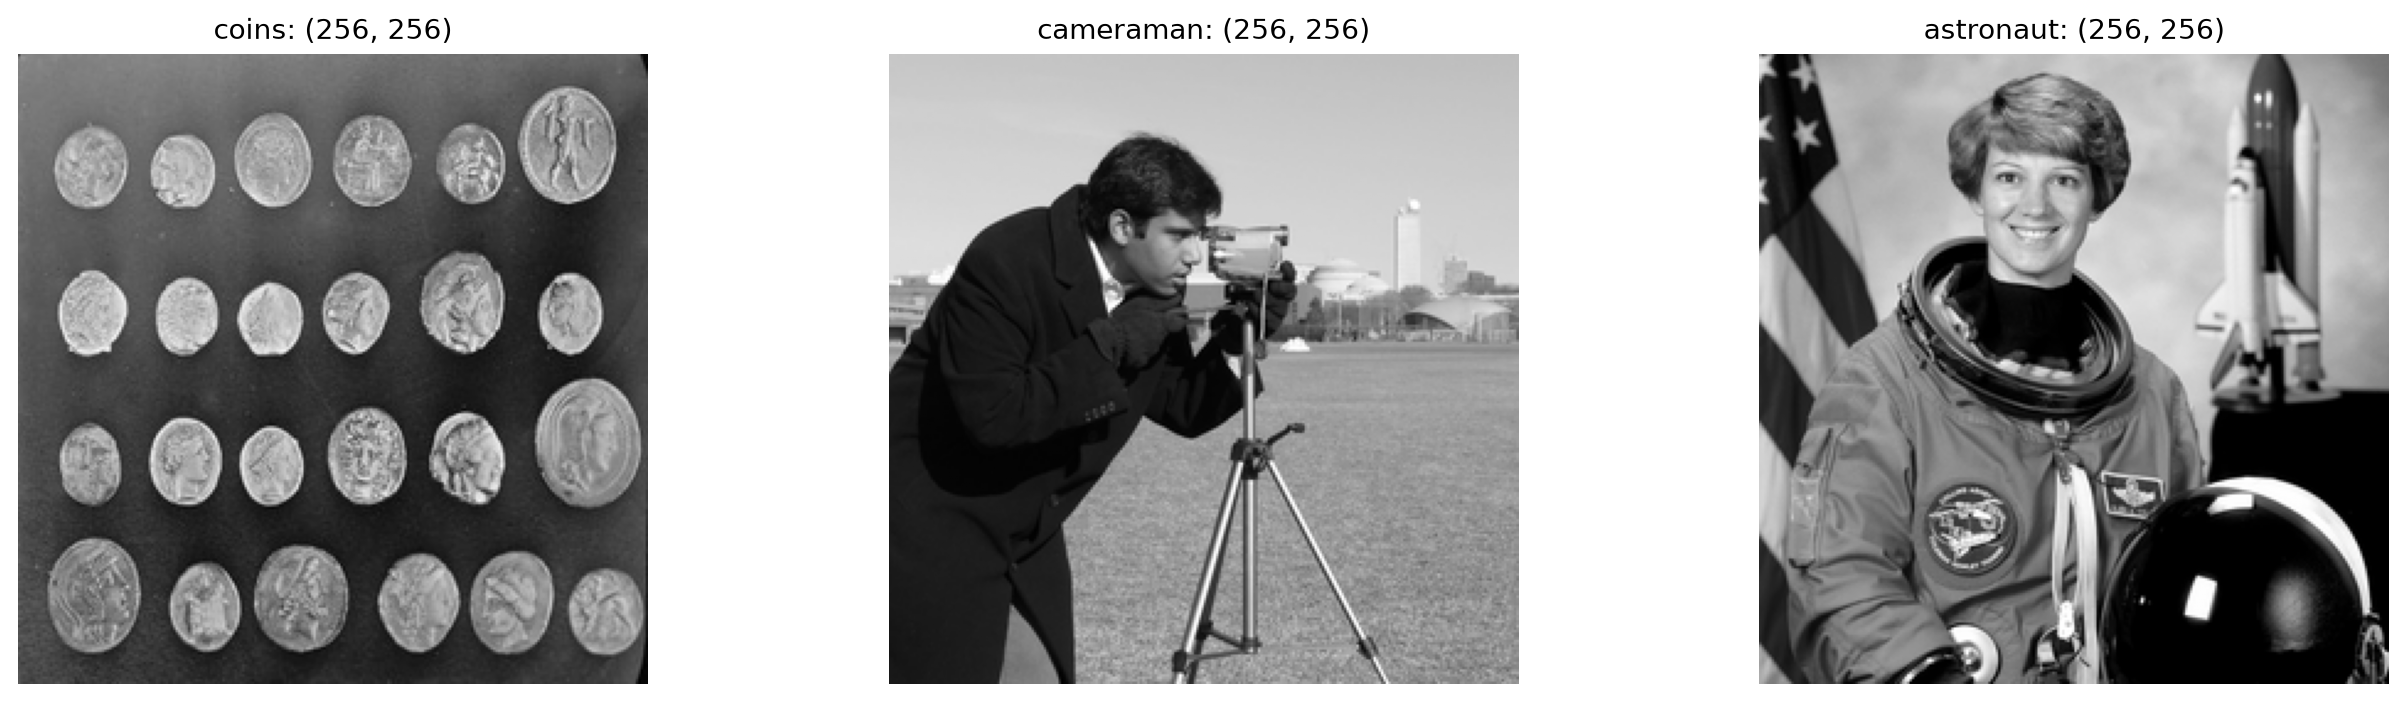
\includegraphics[width=\linewidth]{imagenes_entrada.png}
    \caption{Imágenes de entrada después de la conversión a escala de grises y el redimensionamiento a $256\times256$.}
    \label{fig:entradas}
\end{figure}

\begin{table}[H]
\centering
\caption{Configuración general del experimento.}
\label{tab:configuracion}
\small
\begin{tabular}{>{\raggedright\arraybackslash}p{0.35\linewidth}p{0.52\linewidth}}
\toprule
Elemento & Configuración \\
\midrule
Imágenes & \texttt{coins}, \textit{cameraman} y \texttt{astronaut} \\
Fuente de datos & \texttt{skimage.data} \\
Representación & Escala de grises, valores en $[0,1]$ \\
Resolución de trabajo & $256\times256$ píxeles \\
Coeficientes por imagen & $65\,536$ \\
Bases & Haar-2D de 4 niveles y DCT-2D ortonormal \\
Porcentajes conservados & $5\%$, $10\%$, $20\%$ y $50\%$ \\
Métricas & MSE y PSNR, con rango dinámico 1 \\
\bottomrule
\end{tabular}
\end{table}

\subsection{Flujo de cálculo}

Para cada imagen se realizan los siguientes pasos:
\begin{enumerate}[label=\arabic*.]
    \item calcular los coeficientes Haar y DCT;
    \item vectorizar cada matriz y ordenar $|\theta|$ de mayor a menor;
    \item calcular $E(k)$ y los porcentajes necesarios para 90\%, 95\% y 99\% de energía;
    \item para cada $P$, conservar los $K=\lceil Pn/100\rceil$ coeficientes de mayor magnitud;
    \item aplicar la transformación inversa;
    \item recortar la reconstrucción al intervalo $[0,1]$ y calcular MSE y PSNR.
\end{enumerate}

La función de umbral duro utilizada es:
\begin{lstlisting}[caption={Eliminación de los coeficientes de menor magnitud.},label={lst:threshold}]
def eliminate_coefficients(theta, P):
    theta = np.asarray(theta, dtype=np.float64).ravel()
    if not 0 < P <= 100:
        raise ValueError("P debe estar en el intervalo (0, 100].")
    K = max(1, int(np.ceil(P * theta.size / 100)))
    largest = np.argsort(np.abs(theta))[::-1][:K]
    sparse_theta = np.zeros_like(theta)
    sparse_theta[largest] = theta[largest]
    return sparse_theta
\end{lstlisting}

\subsection{Métricas de reconstrucción}

Para una referencia $x$ y una reconstrucción $\hat{x}$, el error cuadrático medio es
\begin{equation}
    \operatorname{MSE}(x,\hat{x})=\frac{1}{n}
    \sum_{i=1}^{n}(x_i-\hat{x}_i)^2.
    \label{eq:mse}
\end{equation}
Como las imágenes están normalizadas a $[0,1]$, se utiliza $MAX_I=1$ y
\begin{equation}
    \operatorname{PSNR}(x,\hat{x})=10\log_{10}\left(
    \frac{1}{\operatorname{MSE}(x,\hat{x})}\right)\ [\mathrm{dB}].
    \label{eq:psnr}
\end{equation}
Un MSE menor produce un PSNR mayor. Para una base ortonormal, si no se recortaran los valores de la reconstrucción, el error cuadrático total del truncamiento sería igual a la energía de los coeficientes descartados. El recorte a $[0,1]$ se aplica solo para evaluar una imagen válida y puede modificar levemente esa igualdad.

\section{Resultados}

\subsection{Validación de las transformaciones}

Antes del truncamiento se aplicó cada transformación y su inversa. La Tabla~\ref{tab:inversion} muestra el máximo error absoluto. Los valores del orden de $10^{-15}$ corresponden a redondeo de doble precisión y confirman que las reconstrucciones posteriores no están afectadas por un error de implementación.

\begin{table}[H]
\centering
\caption{Error máximo absoluto de inversión para las imágenes completas.}
\label{tab:inversion}
\small
\begin{tabular}{lcc}
\toprule
Imagen & Haar inversa & DCT inversa \\
\midrule
\texttt{coins} & $1.44\times10^{-15}$ & $7.77\times10^{-16}$ \\
\textit{cameraman} & $1.67\times10^{-15}$ & $9.99\times10^{-16}$ \\
\texttt{astronaut} & $1.78\times10^{-15}$ & $8.88\times10^{-16}$ \\
\bottomrule
\end{tabular}
\end{table}

\subsection{Coeficientes ordenados y concentración de energía}

La Figura~\ref{fig:coeficientes} grafica las magnitudes normalizadas de los coeficientes ordenadas de mayor a menor. La escala logarítmica permite observar tanto los coeficientes dominantes como la cola de valores pequeños.

\begin{figure}[H]
    \centering
    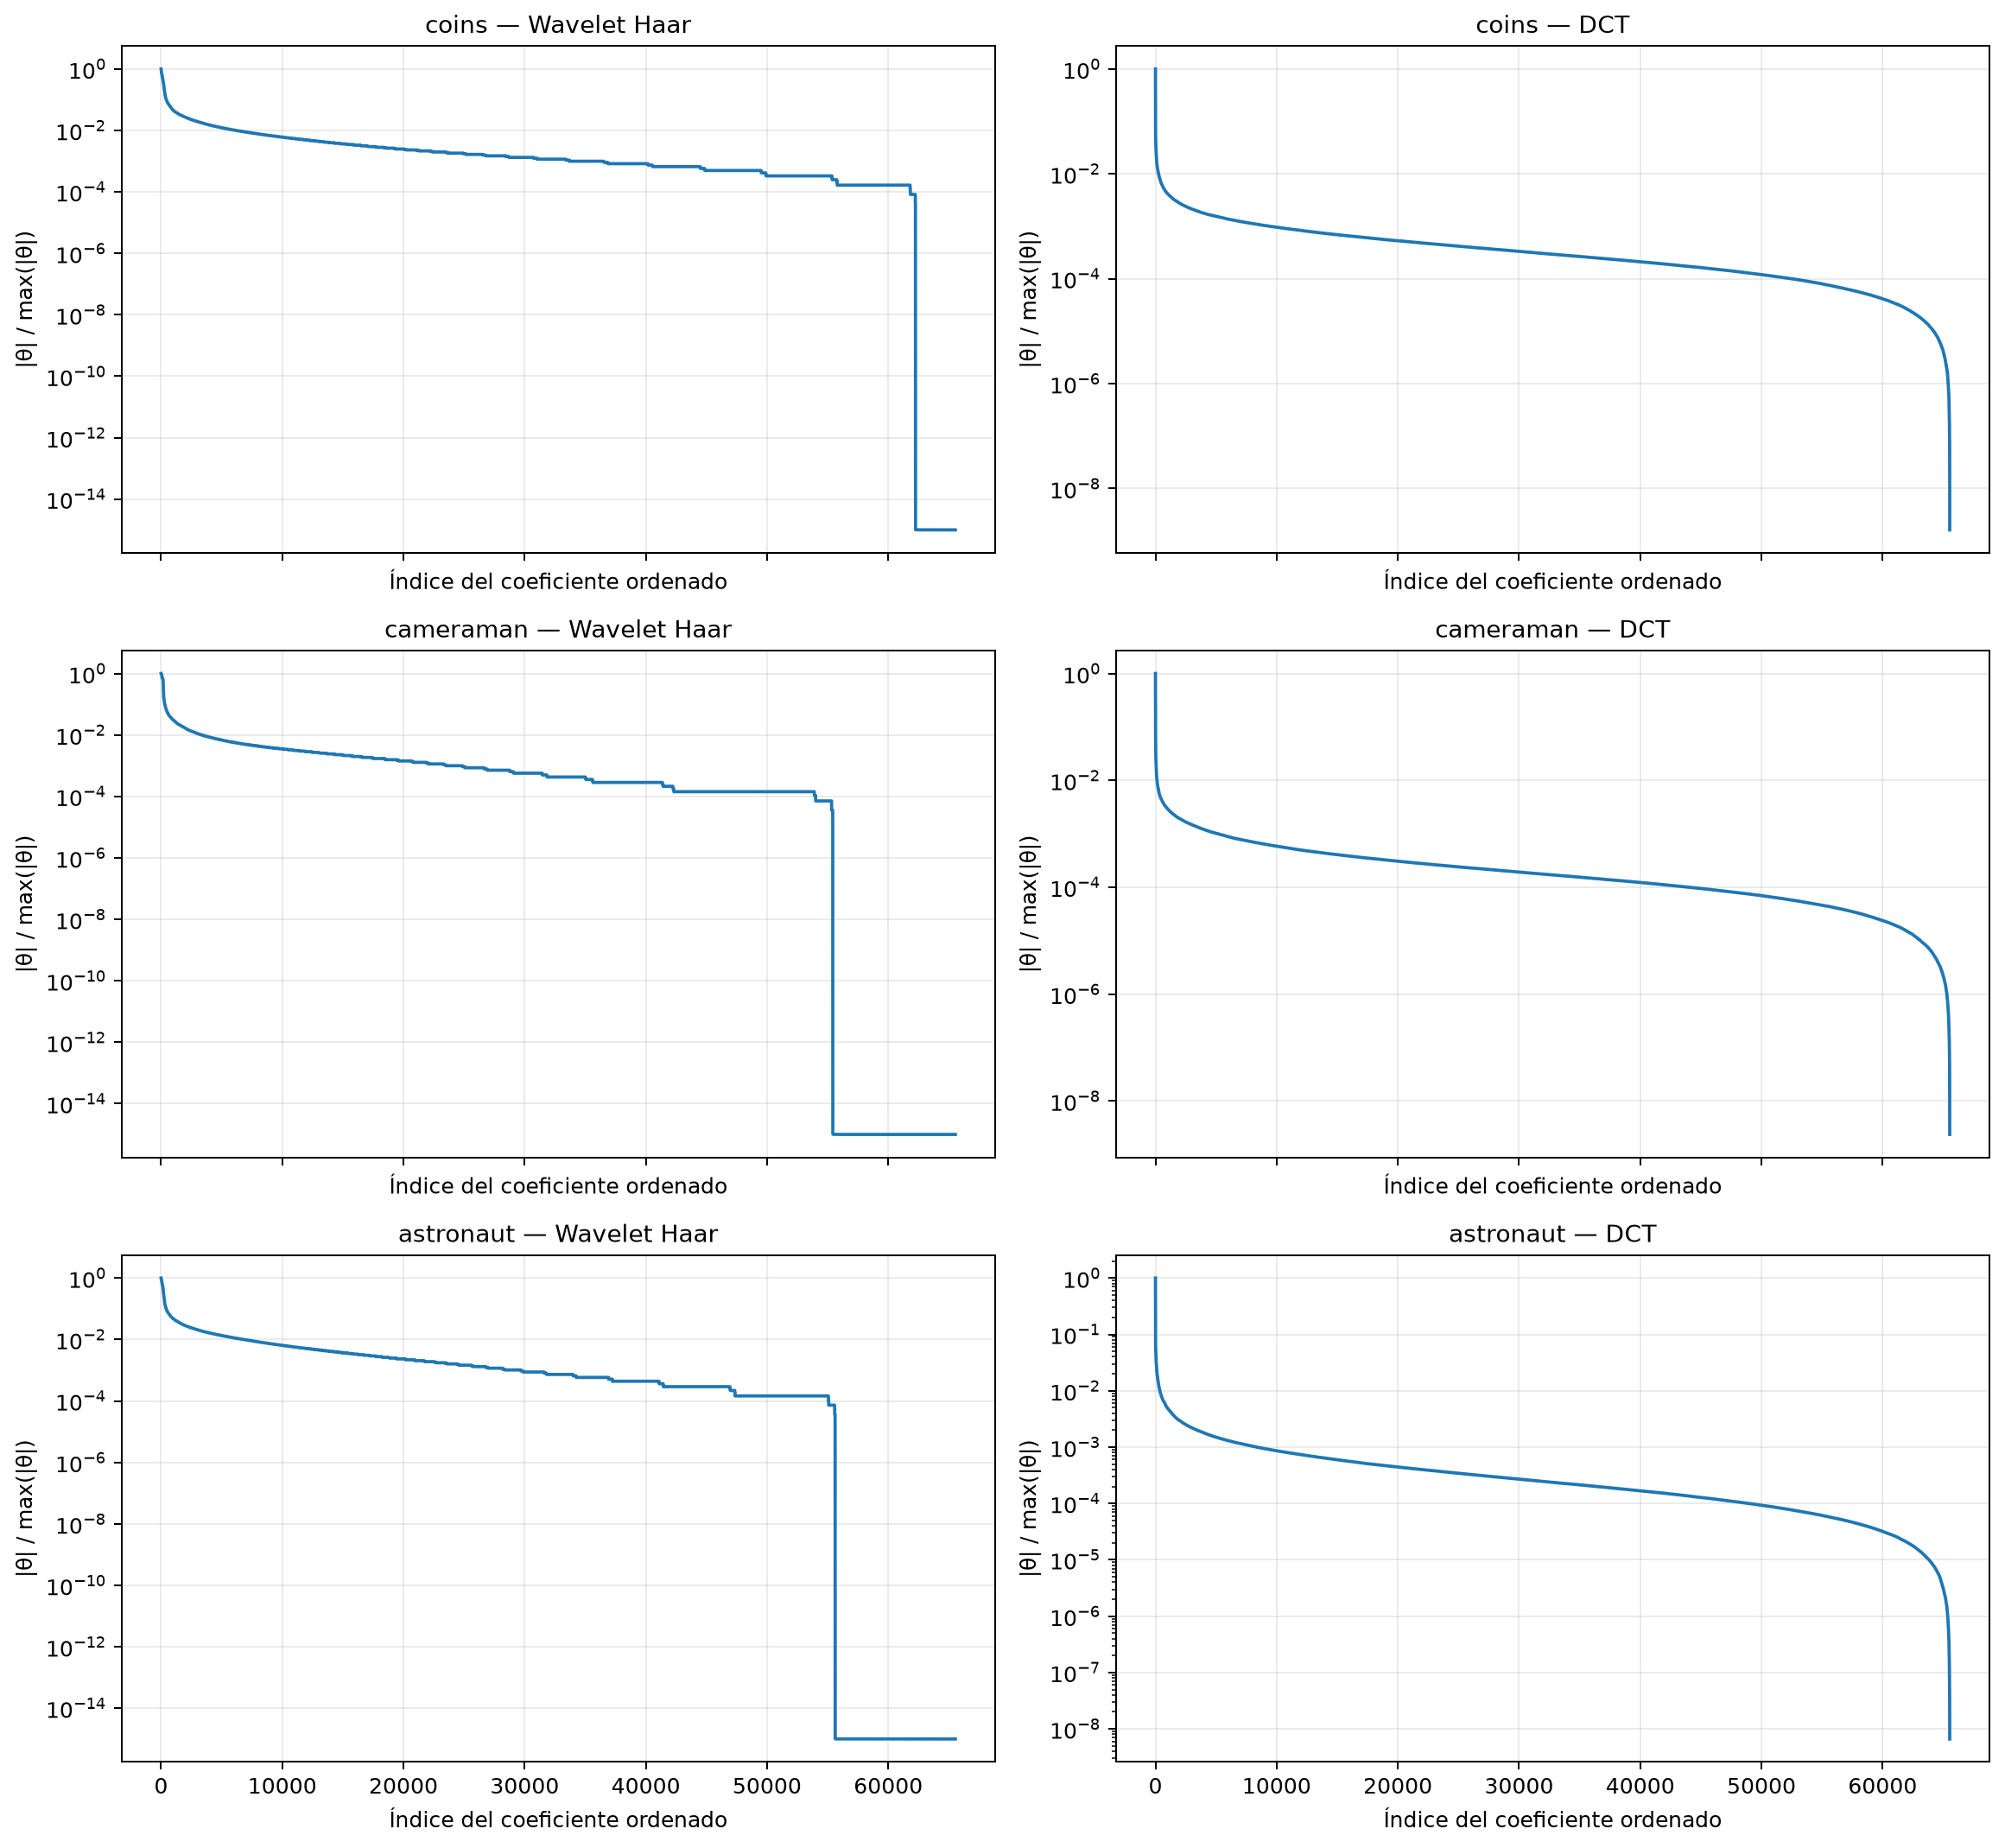
\includegraphics[width=\linewidth]{coeficientes_ordenados.png}
    \caption{Coeficientes ordenados por magnitud para las tres imágenes y las dos bases.}
    \label{fig:coeficientes}
\end{figure}

\begin{table}[H]
\centering
\caption{Energía acumulada y porcentaje de coeficientes necesarios para alcanzar distintos umbrales.}
\label{tab:dispersion}
\scriptsize
\begin{tabular}{llrrrrr}
\toprule
Imagen & Base & 5\% energía & 10\% energía & $k_{90}$ [\%] & $k_{95}$ [\%] & $k_{99}$ [\%]\\
\midrule
\texttt{coins} & Haar & 98.893 & 99.535 & 0.403 & 0.854 & 5.473 \\
\texttt{coins} & DCT & 98.401 & 99.050 & 0.055 & 0.438 & 9.430 \\
\textit{cameraman} & Haar & 99.737 & 99.888 & 0.250 & 0.290 & 1.329 \\
\textit{cameraman} & DCT & 99.381 & 99.663 & 0.009 & 0.041 & 2.460 \\
\texttt{astronaut} & Haar & 98.924 & 99.576 & 0.352 & 0.761 & 5.339 \\
\texttt{astronaut} & DCT & 98.780 & 99.346 & 0.127 & 0.520 & 6.357 \\
\bottomrule
\end{tabular}
\end{table}

Con el criterio del $95\%$ de energía, DCT es la base más compacta en las tres imágenes. Requiere $0.438\%$ de los coeficientes para \texttt{coins}, $0.041\%$ para \textit{cameraman} y $0.520\%$ para \texttt{astronaut}. Sin embargo, al exigir el $99\%$, Haar resulta mejor en los tres casos: $5.473\%$, $1.329\%$ y $5.339\%$, respectivamente, frente a $9.430\%$, $2.460\%$ y $6.357\%$ para DCT.

Este cambio de base ganadora se explica por la cola de coeficientes. La DCT concentra una gran cantidad de energía en los componentes de baja frecuencia, lo que produce una caída inicial muy pronunciada. Haar organiza los detalles de forma localizada y multiescala; aunque puede necesitar más coeficientes para los primeros umbrales, representa de manera eficiente parte de la energía residual asociada a bordes y cambios locales.

\subsection{Reconstrucciones visuales}

El experimento de reconstrucción se ejecutó para las tres imágenes, dos bases y cuatro porcentajes. Las Figuras~\ref{fig:coins-recon}--\ref{fig:astronaut-recon} presentan las galerías generadas por el notebook.

\begin{figure}[H]
    \centering
    \begin{subfigure}{0.49\linewidth}
        \centering
        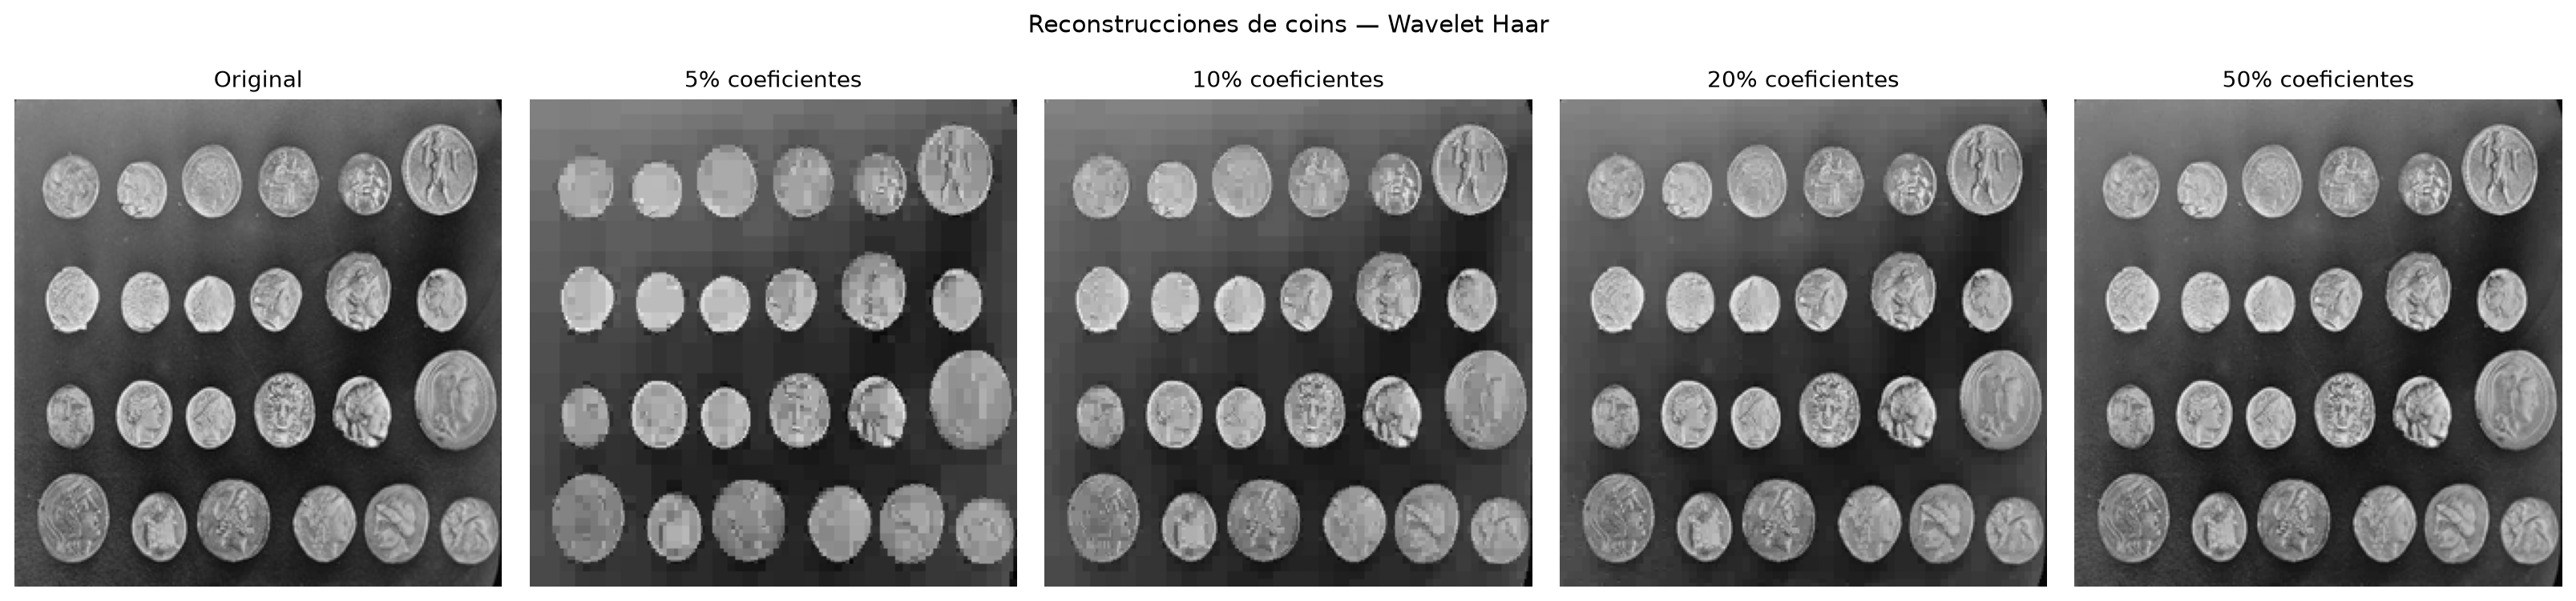
\includegraphics[width=\linewidth]{reconstruccion_coins_haar.png}
        \caption{Haar.}
    \end{subfigure}
    \hfill
    \begin{subfigure}{0.49\linewidth}
        \centering
        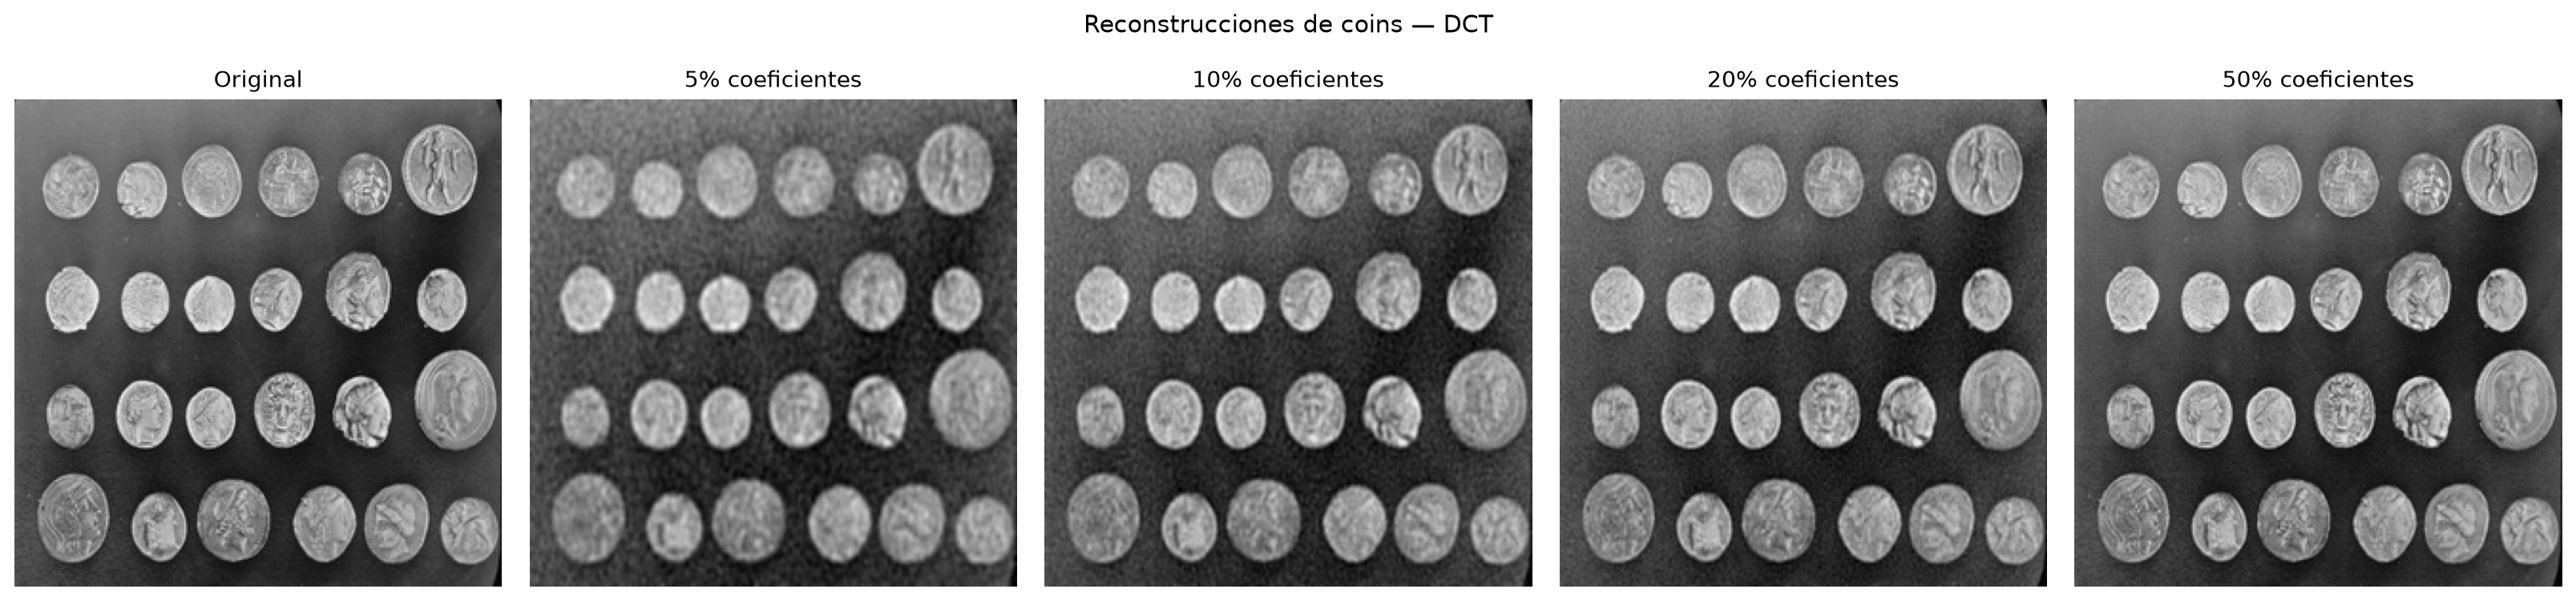
\includegraphics[width=\linewidth]{reconstruccion_coins_dct.png}
        \caption{DCT.}
    \end{subfigure}
    \caption{Reconstrucciones de \texttt{coins} para los cuatro porcentajes de coeficientes.}
    \label{fig:coins-recon}
\end{figure}

\begin{figure}[H]
    \centering
    \begin{subfigure}{0.49\linewidth}
        \centering
        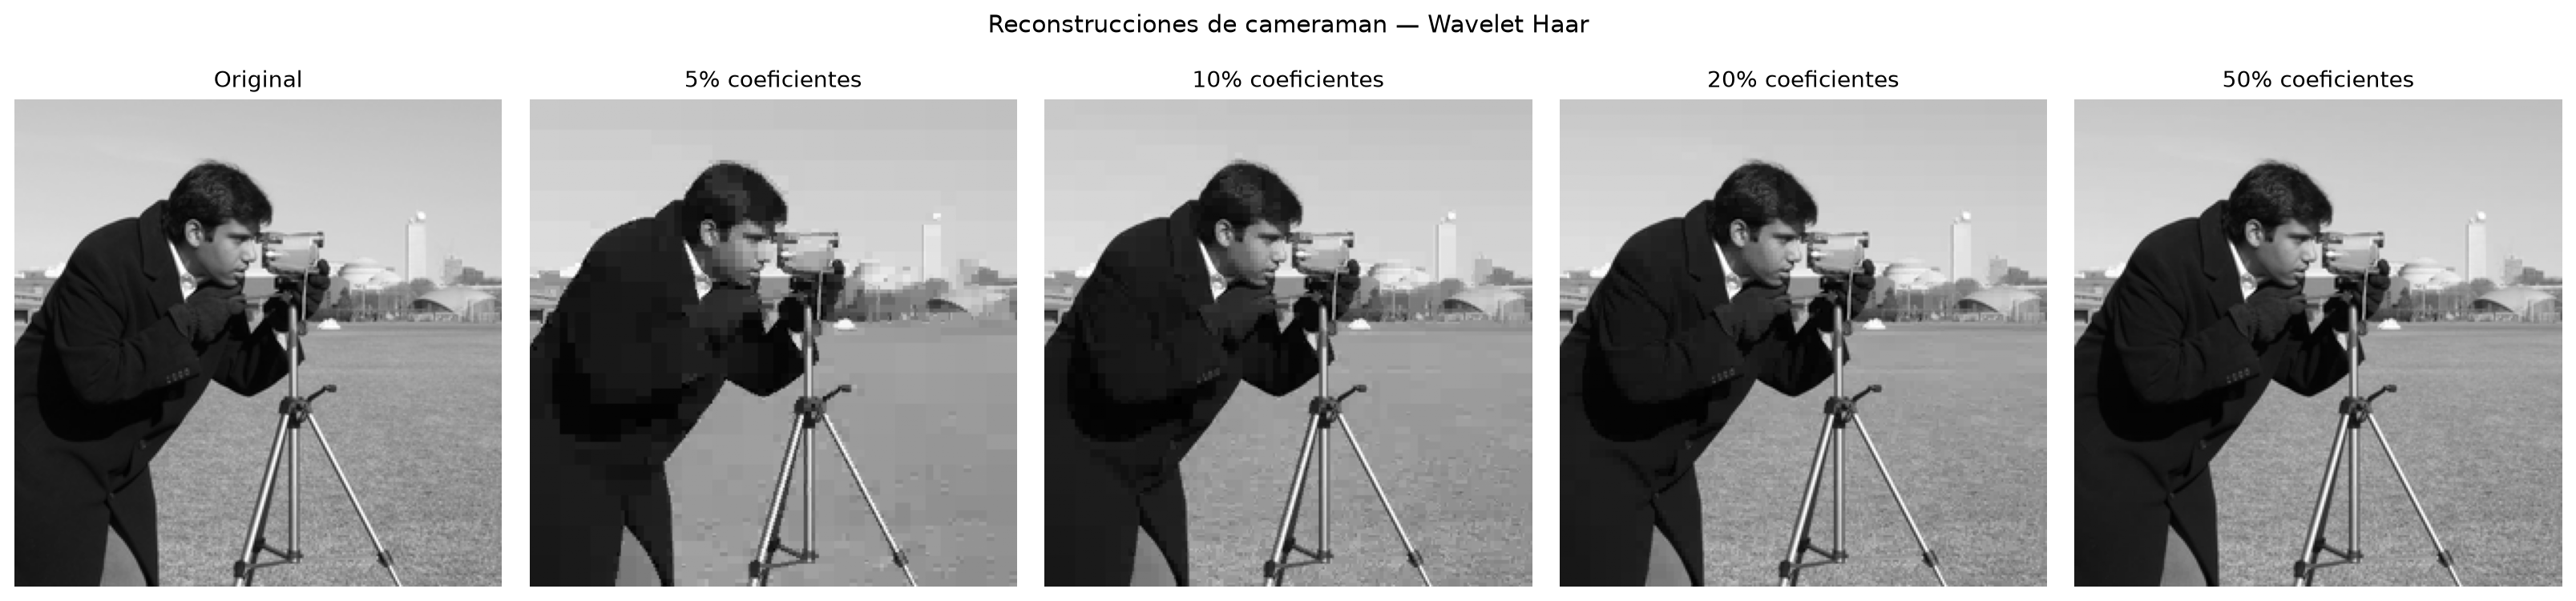
\includegraphics[width=\linewidth]{reconstruccion_cameraman_haar.png}
        \caption{Haar.}
    \end{subfigure}
    \hfill
    \begin{subfigure}{0.49\linewidth}
        \centering
        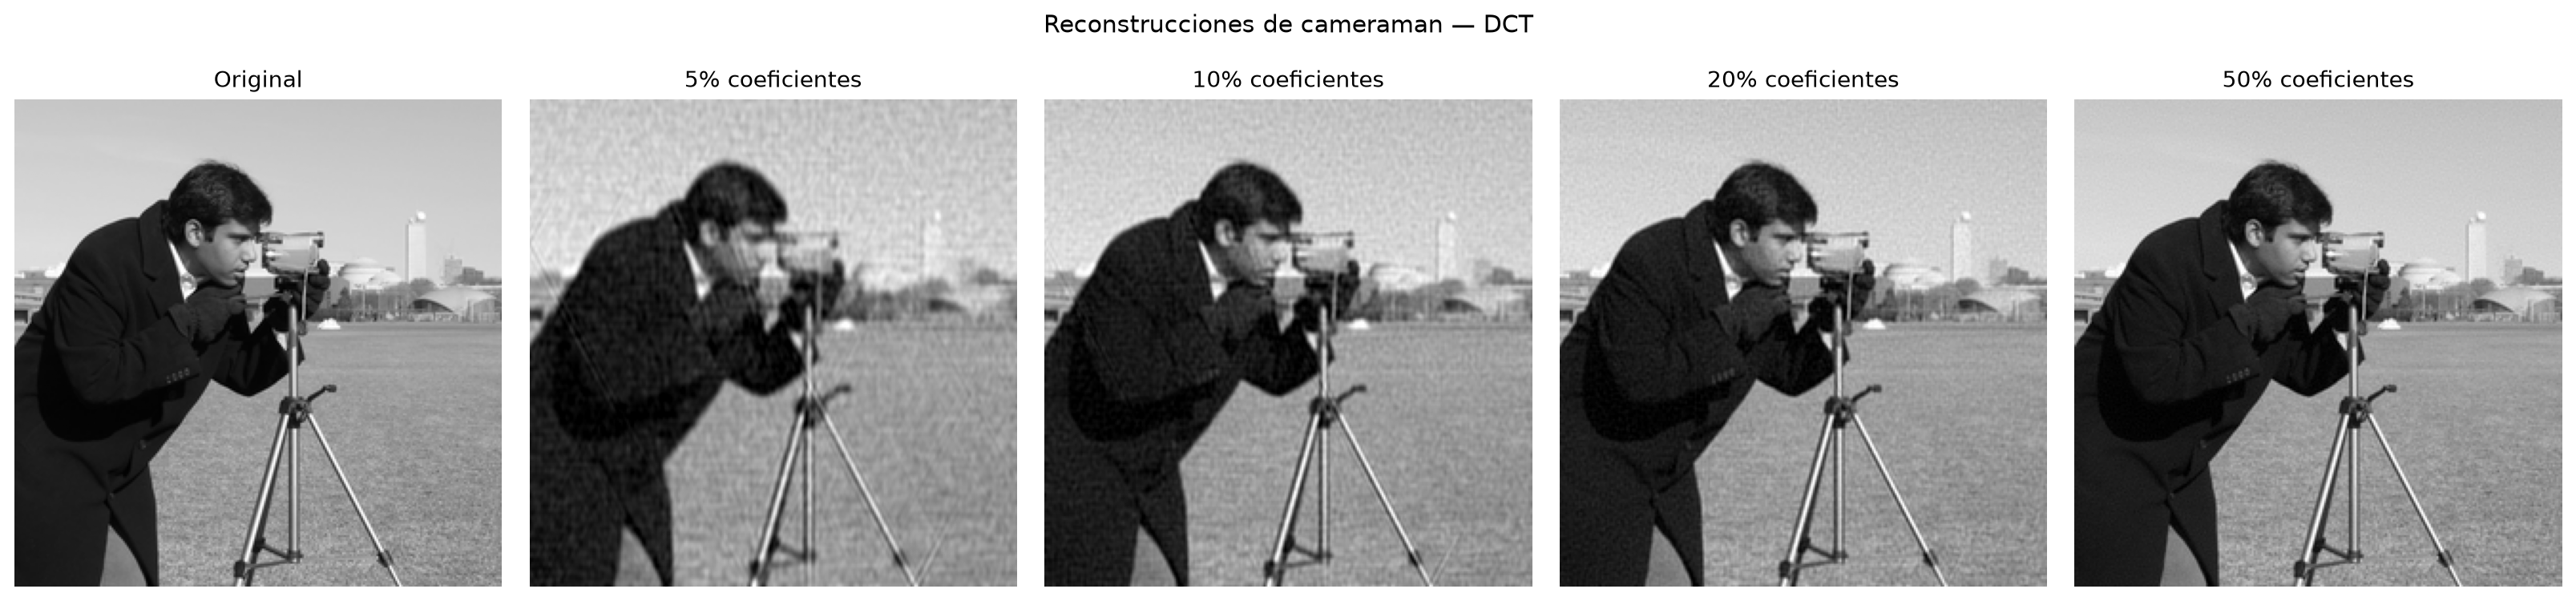
\includegraphics[width=\linewidth]{reconstruccion_cameraman_dct.png}
        \caption{DCT.}
    \end{subfigure}
    \caption{Reconstrucciones de \textit{cameraman} para los cuatro porcentajes de coeficientes.}
    \label{fig:cameraman-recon}
\end{figure}

\begin{figure}[H]
    \centering
    \begin{subfigure}{0.49\linewidth}
        \centering
        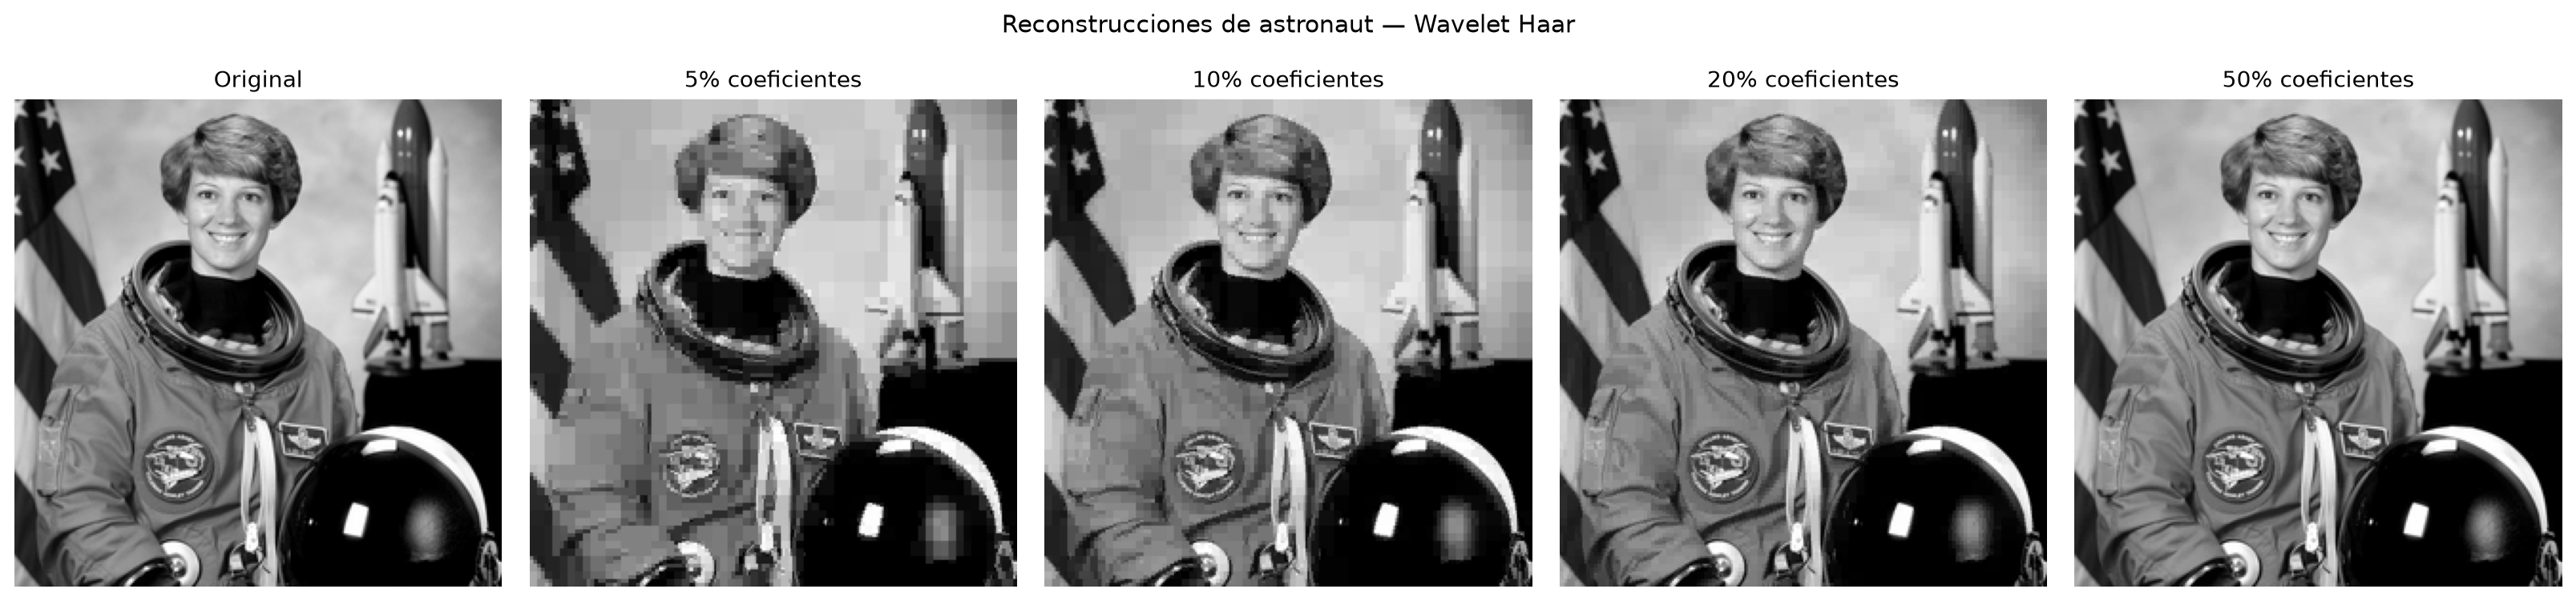
\includegraphics[width=\linewidth]{reconstruccion_astronaut_haar.png}
        \caption{Haar.}
    \end{subfigure}
    \hfill
    \begin{subfigure}{0.49\linewidth}
        \centering
        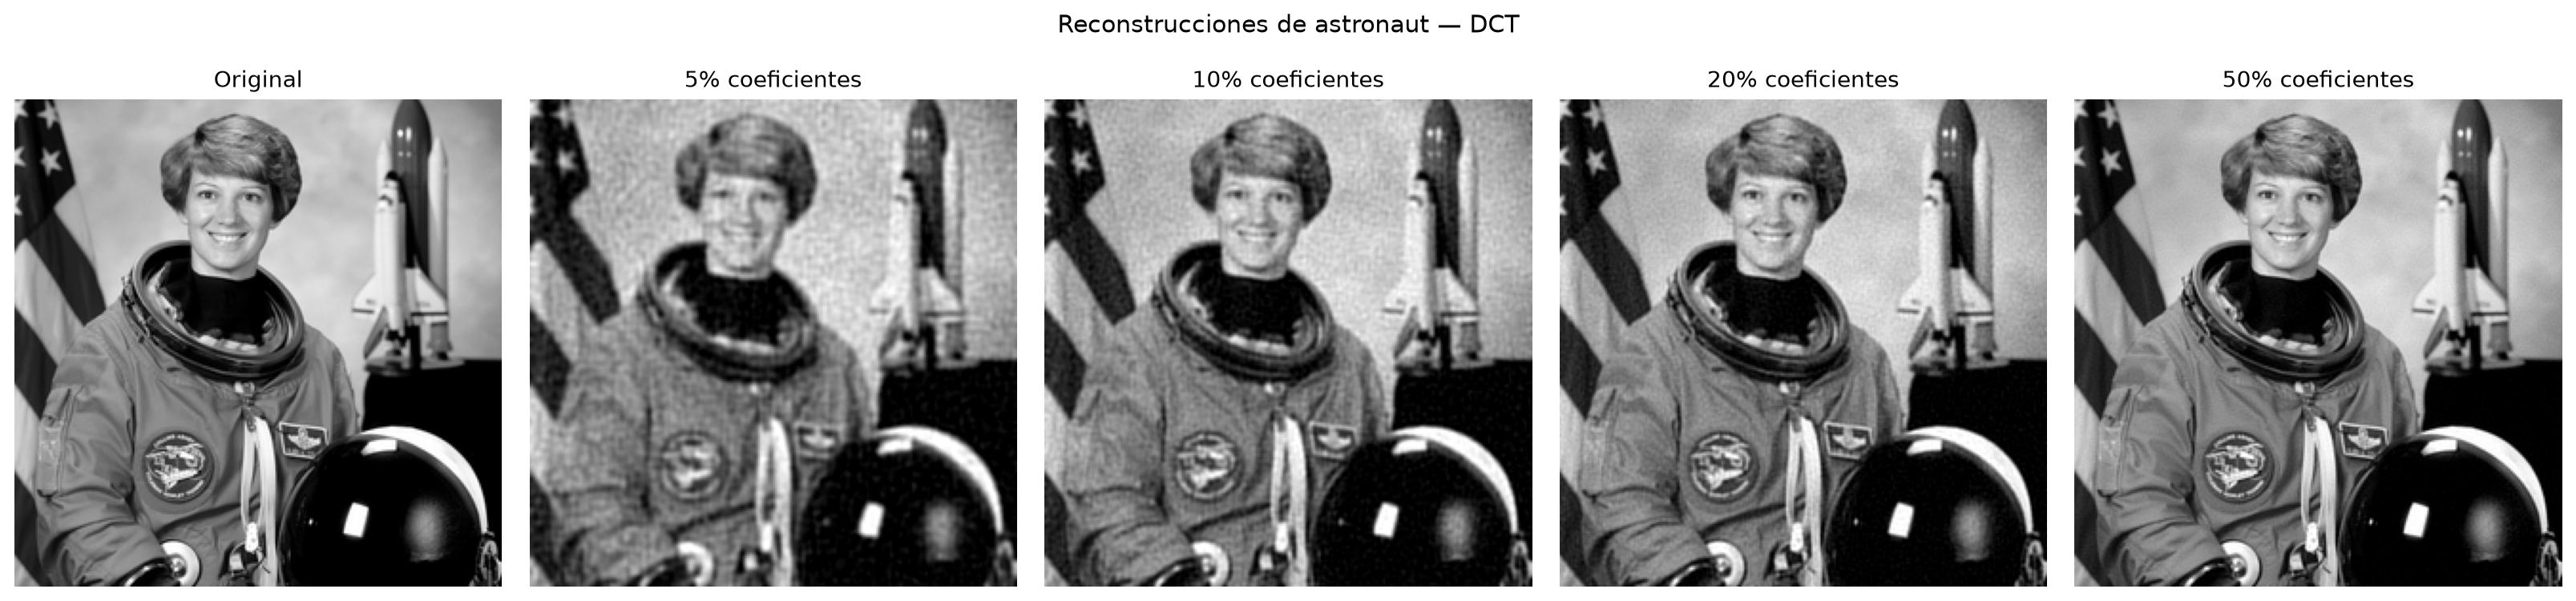
\includegraphics[width=\linewidth]{reconstruccion_astronaut_dct.png}
        \caption{DCT.}
    \end{subfigure}
    \caption{Reconstrucciones de \texttt{astronaut} para los cuatro porcentajes de coeficientes.}
    \label{fig:astronaut-recon}
\end{figure}

En general, con $5\%$ se conservan las estructuras globales, pero se pierden detalles finos. Al aumentar a $10\%$ y $20\%$ se recuperan más bordes y texturas. Con $50\%$ las imágenes resultan visualmente cercanas a la referencia. Haar tiende a mantener cambios locales y bordes, mientras que DCT tiende a producir un suavizado más evidente cuando se eliminan componentes de alta frecuencia.

\subsection{MSE y PSNR para las tres imágenes}

La Tabla~\ref{tab:reconstrucciones} contiene los 24 casos del experimento ampliado. El número de coeficientes conservados es el mismo para ambas bases porque todas las imágenes tienen $n=65\,536$.

\begin{longtable}{llrrrr}
\caption{MSE y PSNR de las reconstrucciones para las tres imágenes.}\label{tab:reconstrucciones}\\
\toprule
Imagen & Base & $P$ [\%] & $K$ & MSE & PSNR [dB]\\
\midrule
\endfirsthead
\toprule
Imagen & Base & $P$ [\%] & $K$ & MSE & PSNR [dB]\\
\midrule
\endhead
\texttt{coins} & Haar & 5 & 3\,277 & $2.060\times10^{-3}$ & 26.86 \\
\texttt{coins} & Haar & 10 & 6\,554 & $8.679\times10^{-4}$ & 30.62 \\
\texttt{coins} & Haar & 20 & 13\,108 & $2.627\times10^{-4}$ & 35.80 \\
\texttt{coins} & Haar & 50 & 32\,768 & $2.268\times10^{-5}$ & 46.44 \\
\texttt{coins} & DCT & 5 & 3\,277 & $2.981\times10^{-3}$ & 25.26 \\
\texttt{coins} & DCT & 10 & 6\,554 & $1.771\times10^{-3}$ & 27.52 \\
\texttt{coins} & DCT & 20 & 13\,108 & $8.251\times10^{-4}$ & 30.83 \\
\texttt{coins} & DCT & 50 & 32\,768 & $1.157\times10^{-4}$ & 39.37 \\
\midrule
\textit{cameraman} & Haar & 5 & 3\,277 & $8.872\times10^{-4}$ & 30.52 \\
\textit{cameraman} & Haar & 10 & 6\,554 & $3.786\times10^{-4}$ & 34.22 \\
\textit{cameraman} & Haar & 20 & 13\,108 & $1.124\times10^{-4}$ & 39.49 \\
\textit{cameraman} & Haar & 50 & 32\,768 & $3.581\times10^{-6}$ & 54.46 \\
\textit{cameraman} & DCT & 5 & 3\,277 & $2.085\times10^{-3}$ & 26.81 \\
\textit{cameraman} & DCT & 10 & 6\,554 & $1.134\times10^{-3}$ & 29.45 \\
\textit{cameraman} & DCT & 20 & 13\,108 & $4.963\times10^{-4}$ & 33.04 \\
\textit{cameraman} & DCT & 50 & 32\,768 & $6.939\times10^{-5}$ & 41.59 \\
\midrule
\texttt{astronaut} & Haar & 5 & 3\,277 & $3.010\times10^{-3}$ & 25.21 \\
\texttt{astronaut} & Haar & 10 & 6\,554 & $1.190\times10^{-3}$ & 29.25 \\
\texttt{astronaut} & Haar & 20 & 13\,108 & $2.897\times10^{-4}$ & 35.38 \\
\texttt{astronaut} & Haar & 50 & 32\,768 & $8.766\times10^{-6}$ & 50.57 \\
\texttt{astronaut} & DCT & 5 & 3\,277 & $3.335\times10^{-3}$ & 24.77 \\
\texttt{astronaut} & DCT & 10 & 6\,554 & $1.776\times10^{-3}$ & 27.51 \\
\texttt{astronaut} & DCT & 20 & 13\,108 & $7.469\times10^{-4}$ & 31.27 \\
\texttt{astronaut} & DCT & 50 & 32\,768 & $9.384\times10^{-5}$ & 40.28 \\
\bottomrule
\end{longtable}

El MSE disminuye y el PSNR aumenta al elevar $P$ en todos los casos. Para \textit{cameraman} y \texttt{astronaut}, Haar supera a DCT en los cuatro porcentajes. En \texttt{coins}, DCT obtiene una ventaja pequeña con $5\%$ y $10\%$, pero Haar es superior con $20\%$ y $50\%$.

La Figura~\ref{fig:psnr} resume esta tendencia. Cada panel corresponde a una imagen y compara la calidad de ambas bases bajo el mismo porcentaje de coeficientes conservados.

\begin{figure}[H]
    \centering
    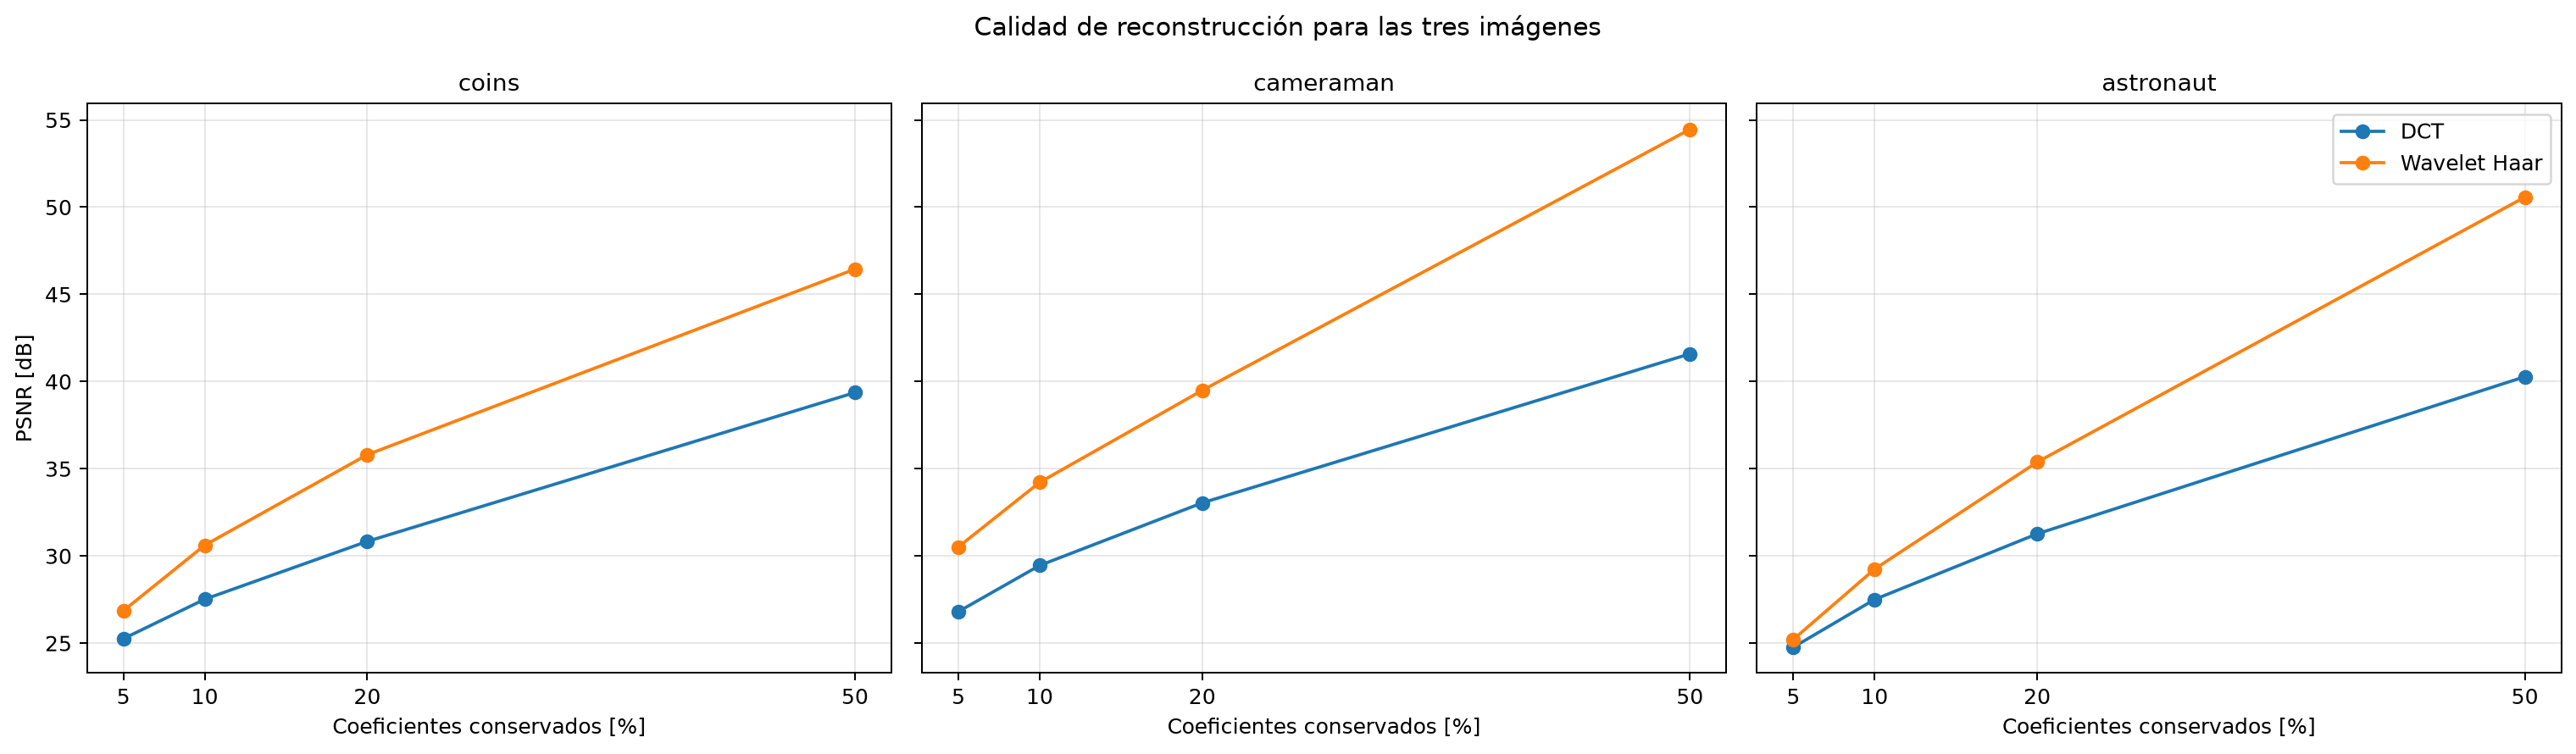
\includegraphics[width=\linewidth]{psnr_tres_imagenes.png}
    \caption{PSNR en función del porcentaje de coeficientes conservados para las tres imágenes.}
    \label{fig:psnr}
\end{figure}

\subsection{Comparación ampliada mediante zoom}

Para complementar la tabla de métricas se inspeccionó la región $x=35{:}220$, $y=35{:}220$ de cada imagen, usando la imagen original y las reconstrucciones Haar/DCT con $20\%$ y $50\%$ de coeficientes. La Figura~\ref{fig:zoom} reúne los tres zooms.

\begin{figure}[H]
    \centering
    \begin{subfigure}{0.32\linewidth}
        \centering
        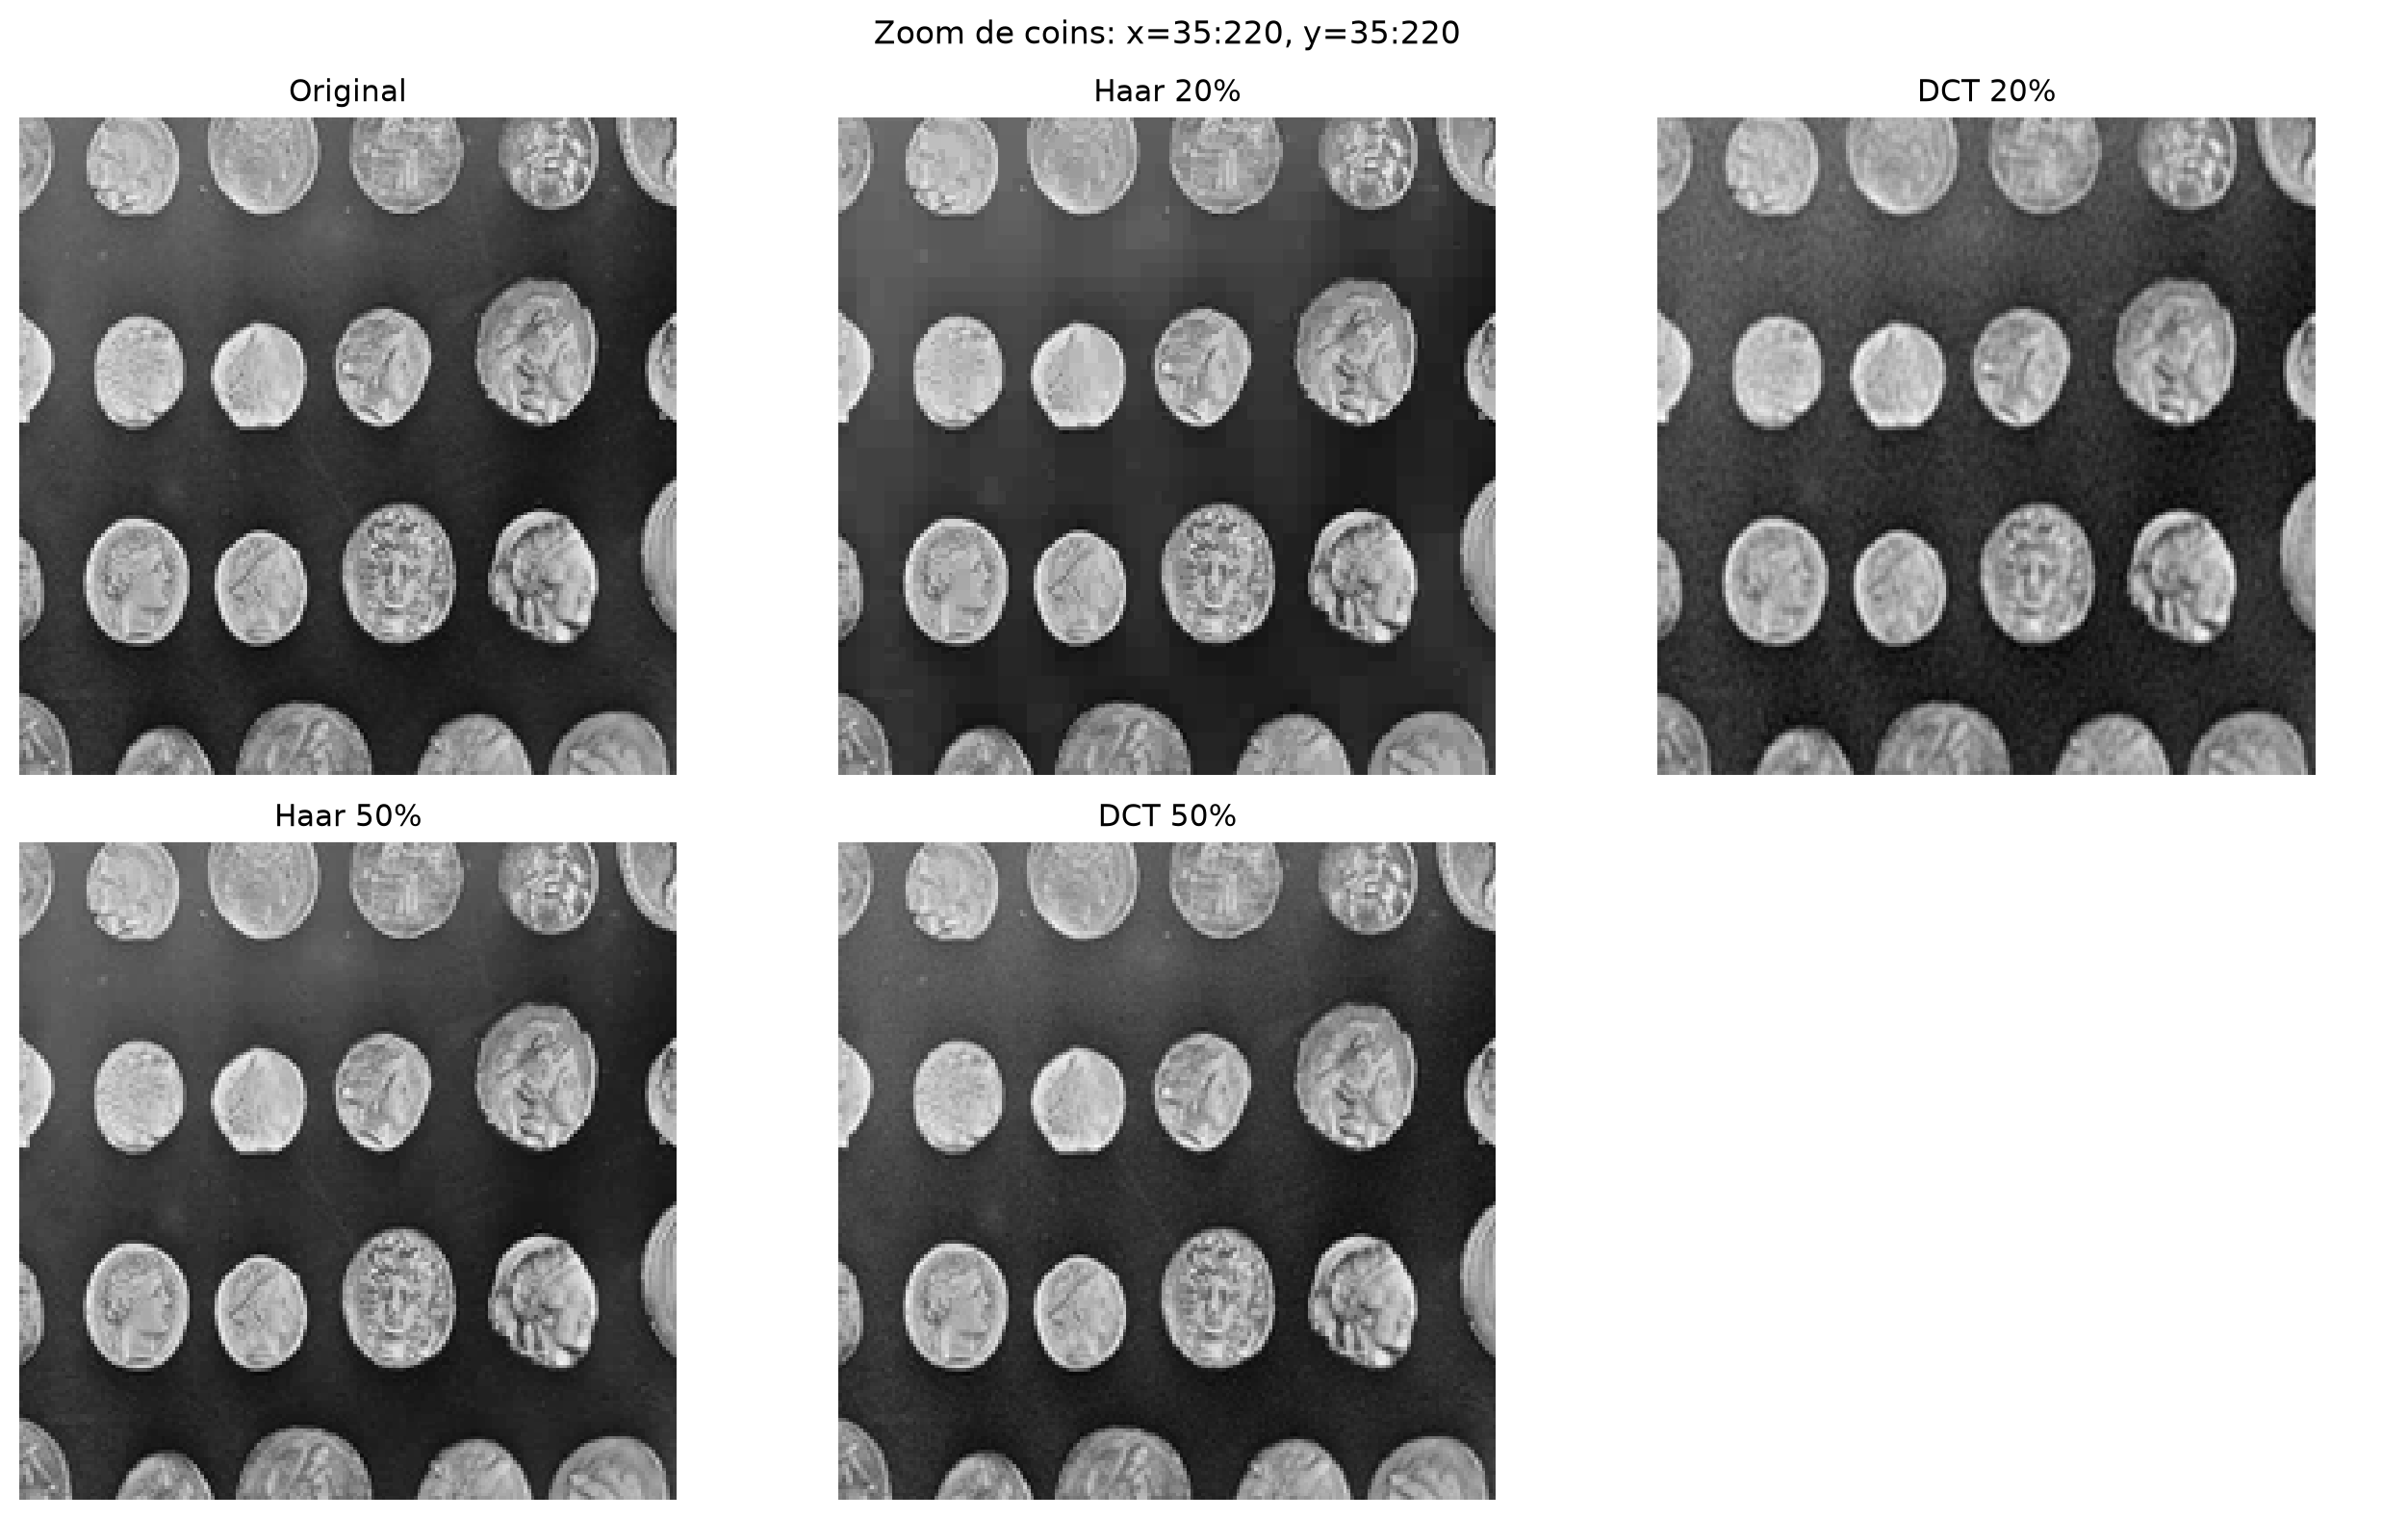
\includegraphics[width=\linewidth]{zoom_coins_comparacion.png}
        \caption{\texttt{coins}.}
    \end{subfigure}
    \hfill
    \begin{subfigure}{0.32\linewidth}
        \centering
        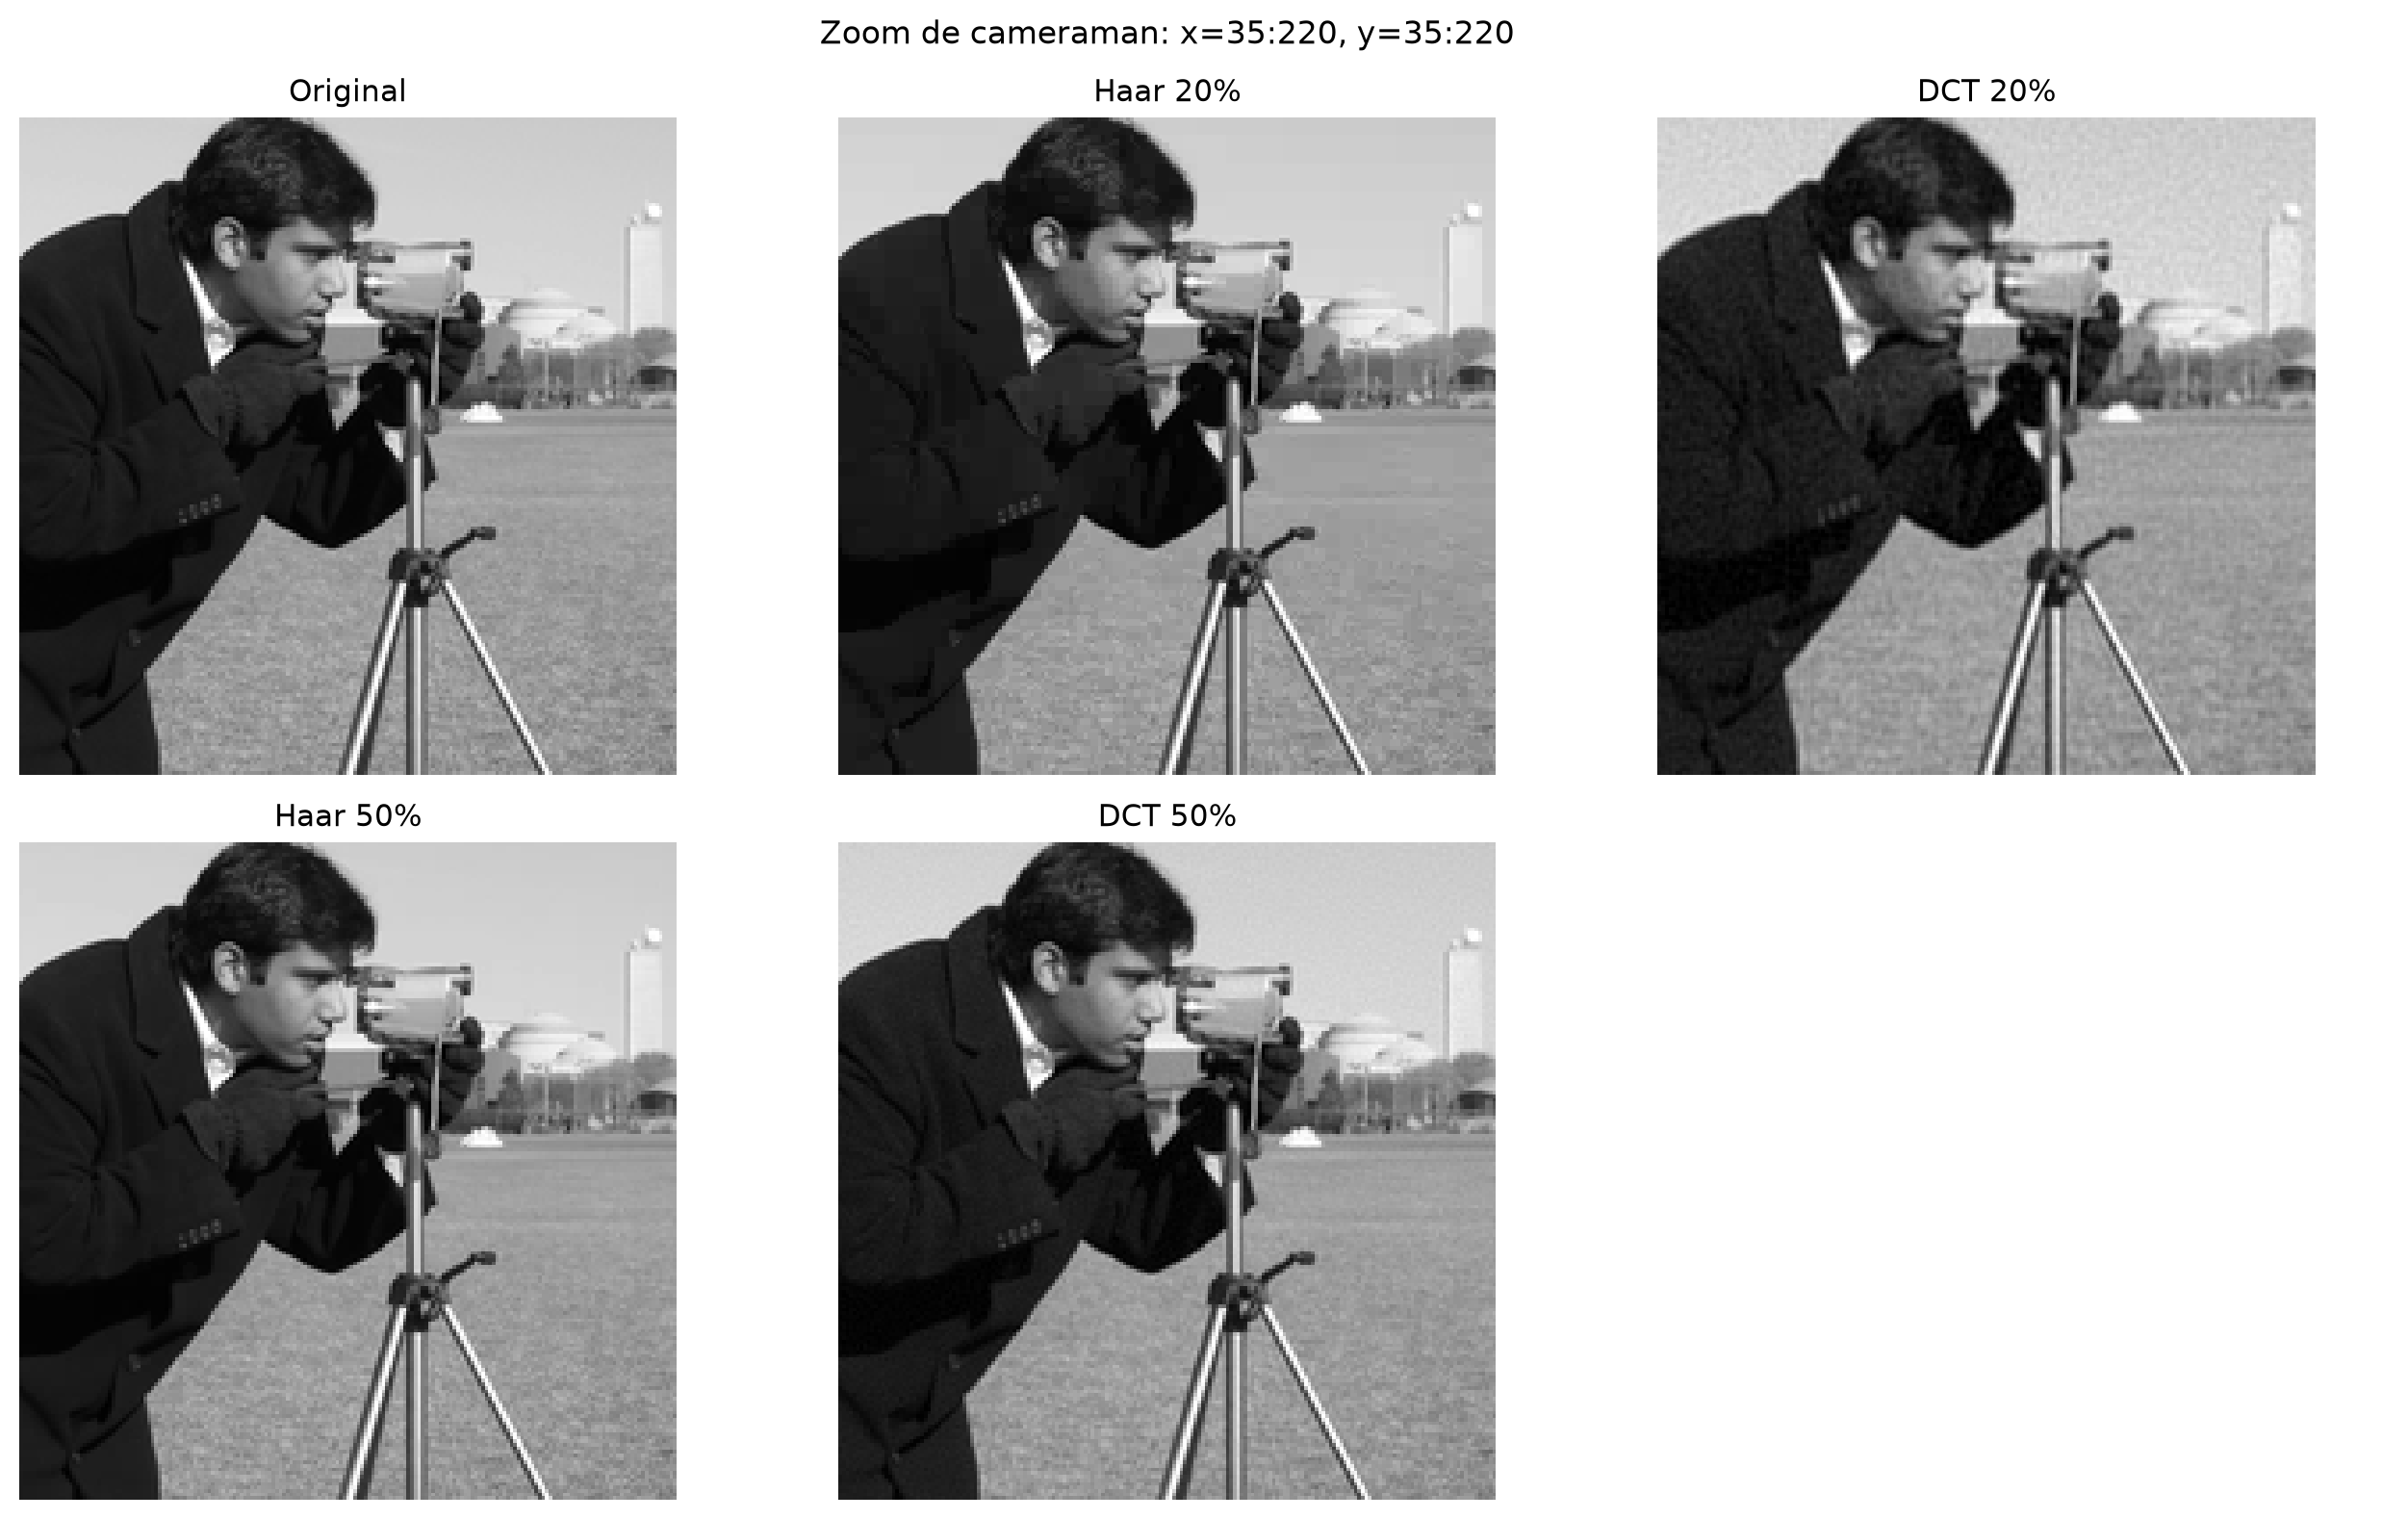
\includegraphics[width=\linewidth]{zoom_cameraman_comparacion.png}
        \caption{\textit{cameraman}.}
    \end{subfigure}
    \hfill
    \begin{subfigure}{0.32\linewidth}
        \centering
        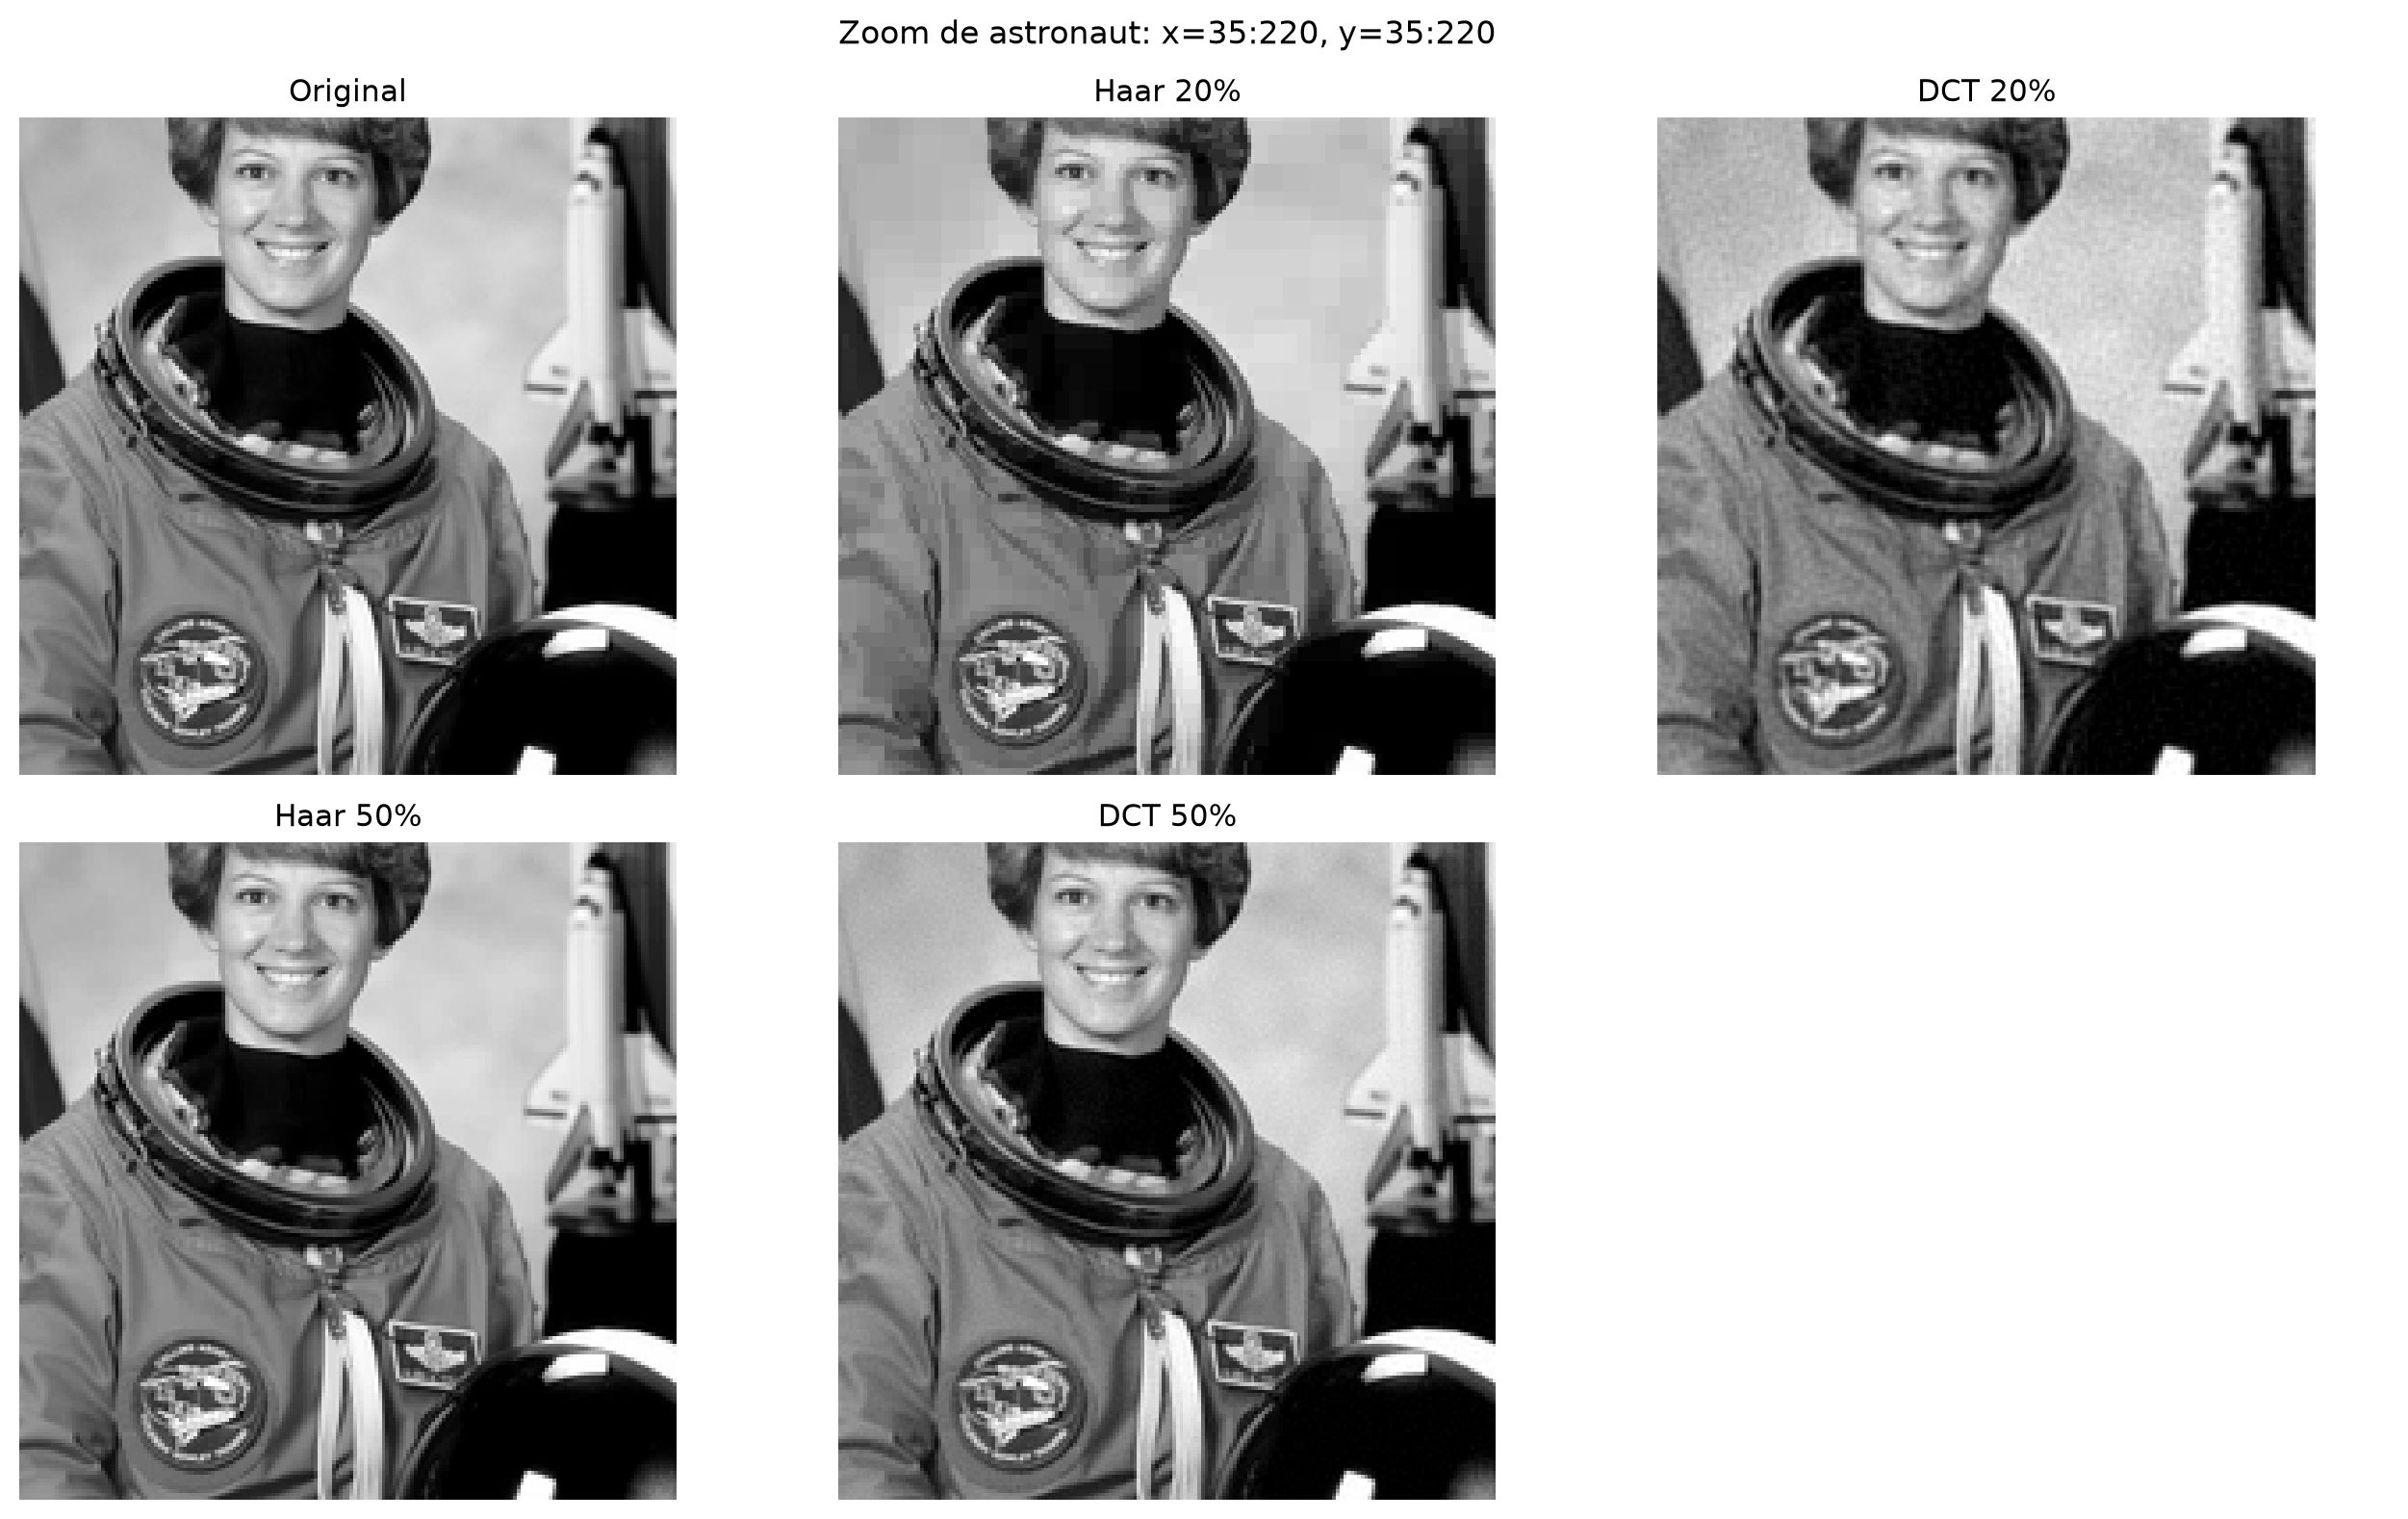
\includegraphics[width=\linewidth]{zoom_astronaut_comparacion.png}
        \caption{\texttt{astronaut}.}
    \end{subfigure}
    \caption{Comparación ampliada de las tres imágenes para porcentajes de $20\%$ y $50\%$.}
    \label{fig:zoom}
\end{figure}

El zoom confirma que el PSNR debe acompañarse con inspección visual. En \textit{cameraman}, Haar conserva con claridad los bordes principales con $20\%$, mientras que DCT suaviza más las transiciones. En \texttt{coins}, DCT puede verse competitivo en los porcentajes más bajos, coherente con su PSNR ligeramente superior a $5\%$ y $10\%$. Con $50\%$, Haar entrega una reconstrucción más nítida en las tres imágenes según las métricas obtenidas.

\section{Discusión}

\subsection{Dos criterios distintos de escasez}

Los resultados muestran que no existe una única respuesta a la pregunta «¿qué base es mejor?». Cuando se fija una fracción de energía, DCT es la más compacta al $95\%$ para las tres imágenes. Cuando se exige $99\%$, Haar resulta más compacta en las tres. Esto ocurre porque las curvas de energía pueden cruzarse: DCT concentra muy bien las componentes principales, mientras que Haar puede representar de mejor manera una parte de los detalles restantes.

Cuando se fija un porcentaje de coeficientes, la pregunta cambia. Ya no se compara cuánta energía captura cada base con el mismo número de coeficientes, sino qué error de imagen produce el truncamiento. Bajo este criterio, Haar gana en diez de los doce pares imagen--porcentaje y DCT gana solo en los dos porcentajes más bajos de \texttt{coins}. La elección de base, por tanto, debe hacerse según la aplicación: almacenamiento muy compacto de la energía dominante y preservación de bordes no son exactamente el mismo objetivo.

\subsection{Relación con el muestreo comprimido}

El esquema de la clase considera una medición $y=A\Psi\theta$. Si $\theta$ tiene pocos elementos significativos y la matriz $A\Psi$ posee suficiente incoherencia o satisface una condición RIP, algoritmos como Orthogonal Matching Pursuit o Iterative Hard Thresholding pueden buscar una solución dispersa. En este informe se aplica únicamente la operación de umbral duro sobre los coeficientes transformados; no se resuelve el problema inverso ni se simula una matriz de medición.

Esta distinción es importante. El experimento demuestra que las imágenes admiten una aproximación con muchos coeficientes nulos en una base transformada, pero no demuestra por sí solo que puedan recuperarse a partir de cualquier conjunto de mediciones. Para estudiar esa etapa habría que definir $A$, analizar el número de mediciones $m$, incorporar ruido y evaluar un algoritmo de recuperación.

\subsection{Limitaciones experimentales}

El redimensionamiento a $256\times256$ facilita la comparación y la descomposición Haar, pero modifica las imágenes originales y puede alterar la distribución de energía. También se utiliza Haar como una elección concreta de Wavelet; otras familias, como Daubechies, podrían representar mejor ciertos tipos de textura. Finalmente, la luminancia de \texttt{astronaut} elimina la información cromática, por lo que el resultado no evalúa la dispersión de sus tres canales RGB por separado.

\section{Conclusiones}

\begin{enumerate}[label=\arabic*.]
    \item Se implementaron y validaron las transformadas Wavelet-2D Haar y DCT-2D. Sus inversas recuperan las tres imágenes con errores del orden de $10^{-15}$.
    \item La DCT es más compacta para alcanzar el $95\%$ de la energía en \texttt{coins}, \textit{cameraman} y \texttt{astronaut}: requiere $0.438\%$, $0.041\%$ y $0.520\%$ de los coeficientes, respectivamente.
    \item Para el $99\%$ de energía, Haar supera a DCT en las tres imágenes: necesita $5.473\%$, $1.329\%$ y $5.339\%$ de los coeficientes.
    \item Al conservar un porcentaje fijo, el MSE disminuye y el PSNR aumenta de forma consistente. Haar entrega el mejor PSNR en todos los casos de \textit{cameraman} y \texttt{astronaut}; en \texttt{coins}, DCT es mejor con $5\%$ y $10\%$, mientras que Haar es mejor con $20\%$ y $50\%$.
    \item La representación más dispersa depende de la imagen, del umbral de energía y del presupuesto de coeficientes. Por ello, no es correcto declarar una base universalmente superior sin especificar el criterio.
    \item El laboratorio proporciona la motivación para el muestreo comprimido: una imagen puede describirse aproximadamente con muchos menos coeficientes significativos que píxeles. La recuperación desde mediciones comprimidas queda como una etapa posterior que requiere definir una matriz $A$ y resolver un problema inverso.
\end{enumerate}

\section{Reproducibilidad y archivos generados}

El c\'odigo se encuentra en \texttt{tareas/tarea-03/homework3.ipynb}. Requiere Python y las bibliotecas NumPy, SciPy, pandas, Matplotlib, Pillow y scikit-image. Si scikit-image no est\'a disponible, el notebook intenta utilizar las im\'agenes de respaldo en \texttt{tareas/dataset/}. Al ejecutar el notebook desde la raiz del repositorio o desde la carpeta de la tarea se generan las figuras y tablas utilizadas en este documento:
\begin{itemize}
    \item \texttt{Fig/imagenes\_entrada.png};
    \item \texttt{Fig/coeficientes\_ordenados.png};
    \item \texttt{Fig/reconstruccion\_<imagen>\_<base>.png};
    \item \texttt{Fig/psnr\_tres\_imagenes.png};
    \item \texttt{Fig/zoom\_<imagen>\_comparacion.png};
    \item \texttt{resultados/dispersion\_por\_imagen.csv};
    \item \texttt{resultados/reconstruccion\_por\_imagen.csv};
    \item un CSV de reconstrucción individual para cada imagen.
\end{itemize}
La tabla principal de reconstrucciones contiene 24 filas: tres imágenes, dos bases y cuatro porcentajes. Las cifras reportadas corresponden a la ejecución que utilizó la fuente oficial \texttt{skimage.data} y la configuración descrita en la Tabla~\ref{tab:configuracion}.

\begin{thebibliography}{9}

\bibitem{lecture}
Nelson Díaz. \textit{Compressive Sensing and Applications, Lecture 3}. Universidad Técnica Federico Santa María, 2026.

\bibitem{book}
David Brady. \textit{Computational Optical Imaging}. SPIE Press, 2025. Seccion 2.5, ``Wavelets'', pp. 41--51; seccion 7.4, ``Compression'', especialmente la discusion de DCT en pp. 424--425.

\bibitem{waveletNotebook}
Arizona Camera Lab. \textit{basesAndWavelets.ipynb}, materiales oficiales del cap\'itulo 2, \texttt{Chapter2ForwardModels}. Repositorio de materiales de \textit{Computational Optical Imaging}.

\bibitem{assignment}
Nelson Díaz. \textit{Muestreo comprimido: Tarea 3, Análisis de Escasez}. Universidad Técnica Federico Santa María, 2 de septiembre de 2026.

\bibitem{dct}
N. Ahmed, T. Natarajan y K. R. Rao. Image coding using the discrete cosine transform. \textit{IEEE Transactions on Computers}, 23(1), 1974.

\bibitem{wavelet}
S. Mallat. A theory for multiresolution signal decomposition: the wavelet representation. \textit{IEEE Transactions on Pattern Analysis and Machine Intelligence}, 11(7), 1989.

\bibitem{skimage}
S. van der Walt et al. scikit-image: image processing in Python. \textit{PeerJ}, 2:e453, 2014.

\end{thebibliography}
\end{document}
